\documentclass[10pt,a4paper]{article}

\usepackage[a4paper,margin=18mm,top=20mm,bottom=21mm,headheight=14pt]{geometry}
\usepackage[T1]{fontenc}
\usepackage[utf8]{inputenc}
\usepackage{mathpazo}
\usepackage{amsmath,amssymb,amsthm,mathtools}
\usepackage{graphicx}
\usepackage{booktabs,tabularx,array}
\usepackage{xcolor}
\usepackage{fancyhdr}
\usepackage{listings}
\usepackage{microtype}
\usepackage{caption}
\usepackage[colorlinks=true,linkcolor=primary,citecolor=tealaccent,urlcolor=primary,
  pdftitle={Trunk and Branches: Thermodynamic Parsimony, Frozen-Core Cortical Columns, and Non-Destructive Continual Specialization via Orthogonal DoRA and Sparsegen LD-MoLE Routing on Consumer Silicon},
  pdfauthor={Lucas Alves Motta (ORCID: 0009-0001-3081-5505)},
  pdfsubject={Technical Monograph and Longitudinal Experimental Audit -- DOI: 10.5281/zenodo.24221509}]{hyperref}

\definecolor{primary}{RGB}{22,50,79}
\definecolor{tealaccent}{RGB}{27,127,121}
\definecolor{goldaccent}{RGB}{175,118,16}
\definecolor{crimsonaccent}{RGB}{162,48,62}
\definecolor{calloutbg}{RGB}{244,248,251}
\definecolor{warmbg}{RGB}{253,249,240}
\definecolor{codebg}{RGB}{248,250,252}
\definecolor{bordergray}{RGB}{205,214,222}
\definecolor{slate}{RGB}{82,96,109}

\setlength{\parskip}{5.2pt plus 1.8pt minus 1pt}
\setlength{\parindent}{0pt}
\renewcommand{\arraystretch}{1.16}
\newcolumntype{Y}{>{\raggedright\arraybackslash}X}
\emergencystretch=1.8em
\captionsetup{font=small,labelfont={bf,color=primary},skip=5pt}

\pagestyle{fancy}
\fancyhf{}
\fancyhead[L]{\footnotesize\color{slate}\textit{Trunk and Branches: Thermodynamic Parsimony \& Non-Destructive Cortical Specialization (Isaque 2.0)}}
\fancyhead[R]{\footnotesize\color{slate}\textit{Motta (2026)}}
\fancyfoot[L]{\footnotesize\color{slate}\textit{Beyond Adonai Monograph --- \href{https://doi.org/10.5281/zenodo.24221509}{\texttt{DOI:\,10.5281/zenodo.24221509}} $\cdot$ BTC Block \#975458}}
\fancyfoot[R]{\footnotesize\color{primary}\textbf{\thepage}}
\renewcommand{\headrulewidth}{0.4pt}
\renewcommand{\footrulewidth}{0.3pt}

\newtheorem{theorem}{Architectural Law}
\newtheorem{proposition}{Empirical Finding}

\newcommand{\insightbox}[2]{%
  \vspace{4pt}\noindent\fcolorbox{primary!45}{calloutbg}{%
    \parbox{\dimexpr\linewidth-2\fboxsep-2\fboxrule\relax}{%
      \vspace{3pt}\textbf{\color{primary}#1.}\hspace{0.4em}#2\vspace{3pt}%
    }%
  }\vspace{4pt}%
}

\newcommand{\auditbox}[2]{%
  \vspace{4pt}\noindent\fcolorbox{goldaccent!70}{warmbg}{%
    \parbox{\dimexpr\linewidth-2\fboxsep-2\fboxrule\relax}{%
      \vspace{3pt}\textbf{\color{goldaccent!90!black}#1.}\hspace{0.4em}#2\vspace{3pt}%
    }%
  }\vspace{4pt}%
}

\lstset{
  basicstyle=\ttfamily\scriptsize,
  backgroundcolor=\color{codebg},
  frame=single,
  rulecolor=\color{bordergray},
  breaklines=true,
  breakatwhitespace=false,
  columns=fullflexible,
  keepspaces=true,
  showstringspaces=false,
  xleftmargin=4pt,
  xrightmargin=4pt,
  aboveskip=5pt,
  belowskip=5pt,
  literate=
    {á}{{\'a}}1 {à}{{\`a}}1 {ã}{{\~a}}1 {â}{{\^a}}1
    {é}{{\'e}}1 {ê}{{\^e}}1 {í}{{\'i}}1 {ó}{{\'o}}1
    {ô}{{\^o}}1 {õ}{{\~o}}1 {ú}{{\'u}}1 {ç}{{\c{c}}}1
    {Á}{{\'A}}1 {É}{{\'E}}1 {Í}{{\'I}}1 {Ó}{{\'O}}1
    {Ú}{{\'U}}1 {Ç}{{\c{C}}}1 {±}{{$\pm$}}1 {≥}{{$\ge$}}1 {≤}{{$\le$}}1
}

\begin{document}

% ==============================================================================
% TITLE & HEADER BLOCK
% ==============================================================================
\thispagestyle{empty}
\begin{center}
  {\footnotesize\color{tealaccent}\textbf{TECHNICAL MONOGRAPH \& LONGITUDINAL EXPERIMENTAL AUDIT $\cdot$ NOVEMBER 2026 (REV.\ 5.0 --- PURE AUDIT EDITION)}}\\[6pt]
  {\LARGE\bfseries\color{primary} Trunk and Branches: Thermodynamic Parsimony, Frozen-Core Cortical Columns, and Non-Destructive Continual Specialization via Orthogonal DoRA and Sparsegen LD-MoLE Routing on Consumer Silicon}\\[8pt]
  {\normalsize\color{slate} A Multi-Month Engineering Chronicle, Step-by-Step Autograd \& Physical Verification Study,\\and Forensic Reproducibility Audit of the \textbf{Isaque 2.0} Cognitive Nervous System}\\[10pt]
  {\normalsize\textbf{Lucas Alves Motta} \hspace{0.35em}{\footnotesize\href{https://orcid.org/0009-0001-3081-5505}{\texttt{ORCID:\,0009-0001-3081-5505}}}}\\
  {\footnotesize Independent Systems Architect \& Principal Investigator, \textit{Beyond Adonai Research Laboratory}, Indaial, Santa Catarina, Brazil}\\
  {\footnotesize Official CERN/Zenodo DOI: \href{https://doi.org/10.5281/zenodo.24221509}{\textbf{\texttt{10.5281/zenodo.24221509}}} $\cdot$ Vault: \href{https://drive.google.com/drive/folders/1xkl3xJ-djEBjyhXbT3oyg7OfOuUbD1lv}{Tese --- Tronco e Ramos} $\cdot$ BTC Block \texttt{\#975458} (\texttt{2026-11-11})}
\end{center}

\vspace{2pt}
\noindent\fcolorbox{primary!35}{calloutbg}{%
  \parbox{\dimexpr\linewidth-2\fboxsep-2\fboxrule\relax}{%
    \vspace{4pt}
    \textbf{\color{primary}Abstract ---} Contemporary artificial intelligence engineering is increasingly governed by monolithic scaling: stacking hundreds of billions of mutable parameters and tens of thousands of raw prompt tokens into continuously resident memory hierarchies. While effective at benchmark saturation, unconstrained monolithic accumulation incurs severe thermodynamic overhead, middle-context attention dilution, and catastrophic interference whenever new procedural skills are trained sequentially. Inspired by the $\approx 20\text{ W}$ metabolic envelope of the human neocortex, avian forebrain neuron-packing density, Jeff Hawkins's Thousand Brains theory of cortical columns, and Niklaus Wirth's principle of lean structural simplicity, this monograph presents the longitudinal design, mathematical formulation, and physical verification of \textbf{Isaque 2.0} (\textit{``Trunk and Branches''}). Rather than modifying a monolithic model, Isaque 2.0 freezes $100\%$ of a hybrid Gated DeltaNet/Attention trunk (\href{https://huggingface.co/Qwen/Qwen3.5-4B}{\texttt{Qwen3.5-4B}}, $d=2560$, $248,320$ tokens, SHA-256 invariant \texttt{c78988d9...2a34}), delegates $\approx 98\%$ of routine system vigilance to zero-VRAM deterministic Rust gates ($<0.5\text{ ms}$ CPU, Split Conformal \texttt{BAVAR} $\ge 0.90$), and materializes specialized procedural knowledge as modular $16.00\text{ MiB}$ cortical cartridges ($\approx 8.38\text{M}$ parameters) stored cold on NVMe SSD at \textbf{$0\text{ MB}$ idle RAM/VRAM}. Across audited execution on a single consumer $8\text{ GB}$ Blackwell GPU (\texttt{NVIDIA GeForce RTX 5060}, $8,151\text{ MiB}$), we report seven primary empirical findings: (1) active 4B inference operates at \textbf{$22.3\text{--}23.3\text{ W}$} and adapter training at \textbf{$28\text{--}31\text{ W}$} with zero residual GPU processes under \texttt{Win32 Job Objects}; (2) a four-stage Windows \texttt{NTAPI} memory pipeline (\texttt{SetProcessWorkingSetSizeEx}, \texttt{VirtualLock}, \texttt{FILE\_\allowbreak{}FLAG\_\allowbreak{}NO\_\allowbreak{}BUFFERING}, \texttt{DiscardVirtualMemory} in $6.61\,\mu\text{s}$) streams a $13.50\text{ GiB}$ MoE pool at $1.75\text{ GiB/s}$ with \textbf{$+0.0039\text{ MiB}$ swap delta}, while proving $100.0\%$ byte-level tokenizer identity ($248,320$ tokens across $68,079$ IDs) with a local $22.02\text{ GB}$ \href{https://huggingface.co/Qwen/Qwen3.5-35B-A3B}{\texttt{Qwen3.5-35B-A3B}} (\texttt{-{}-cpu-moe}, $25.66\text{ tok/s}$) judge; (3) real \texttt{LoRA+} ($\eta_B/\eta_A=6.0$) 32-layer backpropagation at $218\text{--}412\text{ tok/s}$ consolidates private-domain architectural knowledge ($-86.76\%$ cross-entropy loss, $2.429 \to 0.322$, zero subword gluing) under analytical \texttt{Sparsegen} \texttt{LD-MoLE} simplex routing ($g_1=0.5667, g_2=0.4333$, $66$ columns at exact $0.0000$), audited blindly by the $35\text{B}$ critic; (4) early-fusion vision (\texttt{mmproj-BF16}, $449\text{ ms}$) coupled with Tikhonov/InfoNCE Procrustes alignment ($2560 \to 384\text{d}$, $\text{Recall@5}=96.00\%$ on $600$ unseen pairs) lifts Cognitive Conductivity ($\mathrm{ICC}$) by \textbf{$5.43\times$} ($0.5121 \to 2.7828$); (5) in a controlled synaptic ablation across the $19,742$-token \texttt{KEV-1.0} physical verification arena ($0.015\text{ ms}$ \texttt{.mmap} lookup), untaught zero-shot access to the identical \texttt{.mmap} arena scores $0/4$ ($1.77/10$), whereas orthogonal \texttt{DoRA + O-LoRA} ($\|A_2 A_1^\top\|_F^2 = 0.00166$) achieves \textbf{$100\%$ ($4/4$) mechanical approval} in headless \texttt{Blender 5.2.1 LTS} and \texttt{clang++ -std=c++20} ($9.67/10$ blind score, $10.23\times\text{--}11.95\times$ $\mathrm{ICC}$, $0.0\%$ bounding-box error); (6) a $10$-wave continual stress ladder ($H_0\dots H_{10}$) maps monolithic saturation from $100.00\%$ ($k=2$) and \textbf{$98.51\%$ rupture onset ($k=3$)} down to \textbf{$75.31\%$ token accuracy ($31.37\%$ likelihood retention) at $k=10$}, whereas surgical \texttt{LD-MoLE Top-2} with cross-term-free rank concatenation (\texttt{PEFT cat}) and a 3-level \texttt{.mmap} tree preserves \textbf{$100.00\%$ retention across all $10$ waves}; and (7) token-level logit summation across distinct code cartridges induces AST collision (\texttt{SyntaxError}), establishing \textbf{Staged Modular DAG Composition} ($1$ specialist cartridge per stage, $\le 3$ sub-waves per cartridge). All verified tables, discarded intermediate prototypes, pre-registered Stage-2 protocols, SHA-256 manifests, and four Bitcoin blockchain timestamps are openly disclosed.\vspace{3pt}
  }%
}

\vspace{2pt}
{\footnotesize\textbf{\color{primary}Keywords:} Thermodynamic AI $\cdot$ Thousand Brains Cortical Columns $\cdot$ Frozen-Trunk Continual Learning $\cdot$ DoRA \& Orthogonal LoRA (\texttt{O-LoRA}) $\cdot$ Learnable Dynamic Mixture of LoRA Experts (\texttt{LD-MoLE}) $\cdot$ Sparsegen Simplex Routing $\cdot$ Hierarchical \texttt{.mmap} Tree Routing $\cdot$ Physical Code Verification}

\begin{flushright}
{\footnotesize\itshape\color{slate} ``Wisdom is rarely found in the noisy accumulation of an unfinished tower;\\it dwells quietly in the order, parsimony, and faithfulness of small, well-governed foundations.''}
\end{flushright}

\newpage
\tableofcontents
\newpage

% ==============================================================================
% SECTION 1: INTRODUCTION & PHILOSOPHICAL FRAMING
% ==============================================================================
\section{Thermodynamic Parsimony Outperforms Monolithic Accumulation}

Modern machine learning has achieved remarkable breadth through scale, yet its prevailing engineering trajectory exhibits a structural vulnerability that classical computer science diagnosed three decades ago. In \textit{A Plea for Lean Software}, Niklaus Wirth warned that hardware acceleration frequently masks algorithmic bloat until systems collapse under their own coupling complexity \cite{wirth1995lean}. Within artificial intelligence, Schwartz et al.\ formalized the analogous distinction between \textit{Red AI}---which buys marginal accuracy gains through exponential compute, memory, and electricity expenditure---and \textit{Green AI}, which treats efficiency and structural parsimony as first-class scientific metrics \cite{schwartz2020green}.

When organizations attempt to endow one monolithic neural network with every domain skill simultaneously---or inject tens of thousands of heterogeneous specification tokens into every inference prompt---three compounding pathologies emerge, which we collectively term \textbf{the Monolithic Babel Trap}:
\begin{enumerate}
  \item \textbf{Thermodynamic Disproportion:} A continuously resident $30\text{B}\text{--}70\text{B}+$ dense or unpaged model consumes $250\text{--}350\text{ W}$ of desktop GPU power (or kilowatt-scale datacenter slices) even when handling routine orchestration tasks, standing in stark contrast to the human brain's $\approx 20\text{ W}$ total metabolic budget \cite{kandel2021principles,attwell2001energy}, where signaling efficiency requires keeping $\le 15\%$ of cortical neurons simultaneously active.
  \item \textbf{Representational Dilution in Long Contexts:} Flooding a causal decoder with $6,000\text{--}30,000$ raw documentation tokens triggers severe middle-context retrieval degradation (\textit{Lost in the Middle}) \cite{liu2024lost}, inflating Time-To-First-Token (TTFT) and causing small or mid-sized executors to hallucinate API signatures or violate geometric constraints.
  \item \textbf{Catastrophic Subspace Interference:} Continually fine-tuning a single parameter matrix or a single low-rank adapter across sequential task waves overwrites previously consolidated manifolds \cite{kirkpatrick2017ewc,chaudhry2018rwalk}, degrading earlier capabilities long before parameter capacity is nominally exhausted.
\end{enumerate}

Comparative neurobiology offers two constructive counter-models to monolithic brute force. First, Olkowicz et al.\ demonstrated that corvids and parrots achieve primate-like forebrain neuron counts and complex tool-making cognition within a drastically smaller cranial volume via high-density pallial neuron packing \cite{olkowicz2016birds}. Second, as synthesized in Jeff Hawkins's \textit{Thousand Brains Theory} \cite{hawkins2019grid,hawkins2021thousand,clay2024monty} and Daniel Kahneman's dual-process cognition \cite{kahneman2011thinking}, the neocortex does not recompile its foundational sensory-motor trunk to learn a new skill, nor does it fire globally at peak metabolic rate. Instead, intelligence is organized as a stable shared substrate (\textbf{the Trunk}) coupled to thousands of semi-autonomous, sparsely recruited cortical columns (\textbf{the Branches}), coordinated by fast reflex gates (System 1) and deliberate adversarial verification (System 2).

This monograph documents the multi-month research, engineering, and forensic auditing journey that translated these principles into \textbf{Isaque 2.0}, a local cognitive nervous system built on consumer hardware in Indaial, Santa Catarina, Brazil. Conceived not as a rival to cloud foundation models---indeed, its own backbone builds directly upon open foundation weights \cite{qwen35_4b}---but as a disciplined local organism governed by deterministic physical verification, Isaque 2.0 demonstrates that a frozen $4\text{B}$-parameter hybrid trunk (\href{https://huggingface.co/Qwen/Qwen3.5-4B}{\texttt{Qwen3.5-4B}}), paired with $16.00\text{ MiB}$ orthogonal cortical cartridges, zero-copy memory-mapped symbolic grammars (\texttt{KEV-1.0}), four-stage Windows \texttt{NTAPI} memory discipline, and a blind $35\text{B}$ Mixture-of-Experts reviewer (\href{https://huggingface.co/Qwen/Qwen3.5-35B-A3B}{\texttt{Qwen3.5-35B-A3B}}), achieves $100\%$ physical verification accuracy in controlled synaptic ablations and $100.00\%$ continual retention across ten sequential specialization waves while consuming $0\text{ MB}$ of idle VRAM and $22.3\text{--}23.3\text{ W}$ during active inference pulses.

\insightbox{Core Thesis (\textit{Trunk and Branches})}{Lasting capability on constrained silicon comes not from stacking larger monolithic layers, but from architectural parsimony: (i) an immutable language-vision trunk, (ii) deterministic symbolic/AST gates handling $\approx 98\%$ of idle vigilance at zero GPU cost, (iii) orthogonal $16.00\text{ MiB}$ cortical columns routed analytically on the unit simplex (\texttt{LD-MoLE} + 3-level \texttt{.mmap} tree), and (iv) staged modular execution verified against deterministic physical compilers (\texttt{Blender bmesh} and \texttt{clang++ -std=c++20}).}

% ==============================================================================
% SECTION 2: MULTI-MONTH LONGITUDINAL ENGINEERING CHRONICLE
% ==============================================================================
\section{Longitudinal Research Chronicle: From the 20 W Axiom to Blockchain-Anchored Verification}

Scientific transparency requires reporting not only final benchmark peaks, but the chronological path---including falsified hypotheses, compiler deadlocks, and architectural pivots---that produced them. Building upon eleven months of broader multi-agent systems engineering ($\approx 3,800\text{--}4,000$ cumulative bench hours across the \texttt{Abra\~ao} ecosystem) and audited across $77$ immutable ledger entries in \texttt{memoria.jsonl} (\texttt{2026-10-03} to \texttt{2026-11-14}) plus over $9,700$ recorded steps across local workspaces (\texttt{c6571c3b} and \texttt{ce5dabcc}), the focused consolidation of Isaque 2.0 unfolded across seven primary phases (eight chronological milestones) summarized in Table~\ref{tab:chronicle}.

\begin{table}[!htbp]
\centering
\caption{Longitudinal engineering and verification chronicle of the Isaque 2.0 research program (October--November 2026), grounded in local L4 ledgers and canonical Drive archives (\href{https://drive.google.com/drive/folders/1xkl3xJ-djEBjyhXbT3oyg7OfOuUbD1lv}{Tese --- Tronco e Ramos}).}
\label{tab:chronicle}
\footnotesize
\begin{tabularx}{\linewidth}{@{}llY@{}}
\toprule
\textbf{Date Window} & \textbf{Milestone / Phase} & \textbf{Verified Engineering Outcome, Telemetry \& Architectural Pivot} \\
\midrule
Oct 03--06, 2026 & Phase I: \textit{20 W Brain Axiom} \& \texttt{N01--N05} & Full-book synthesis (Hawkins, Kahneman, Kandel, Kleppmann, Blandy, Huyen). Architectural inversion (Oct 06): Isaque defined as an event-driven nervous system sleeping $\approx 98\%$ of the time ($<50$ injected tokens per wake pulse). Module \texttt{N05} sealed in Rust (\texttt{68/68} tests green, commit \texttt{ad819d11}). \\
Oct 07--08, 2026 & Phase IIa: Rust 2024 \& Trunk Selection & Workspace unified on Rust \texttt{1.99} (Edition 2024, single \texttt{libc 0.2.190}, checkpoint \texttt{3198add}) after rejecting CLI wrapper workarounds. Windows physical RAM reader established ($62.76\text{ GiB}$ host vs.\ $31\text{ GiB}$ WSL illusion). Base upgraded from \texttt{Qwen3} to hybrid \href{https://huggingface.co/Qwen/Qwen3.5-4B}{\texttt{Qwen3.5-4B}} (\texttt{rev 851bf6e8}, $248,320$ frozen vocab). \\
Oct 09--25, 2026 & Phase IIb: \texttt{N07--N08} Parity \& Live Daemon & \texttt{N07} sealed (Oct 12): numerical parity \texttt{308/313}, $\mathrm{KL}=0.000243$ vs.\ frozen reference, bilingual PT-BR$\leftrightarrow$EN Tucano normalization ($<0.5\text{ ms}$ CPU), and Split Conformal \texttt{BAVAR} $\ge 0.90$ gate \cite{angelopoulos2023conformal}. \texttt{N08} live Rust server active (Oct 13), establishing $680$-item baseline ($31.76\%$) and \texttt{ORPO} pipeline. \\
Nov 07--09, 2026 & Phase III: Power Telemetry \& Stage 1 Cache & Measured \texttt{RTX 5060} board power (\texttt{faixa-A.json}, Nov 08): \textbf{$22.3\text{--}23.3\text{ W}$} active 4B inference ($3.87\text{ GiB}$ VRAM) and \textbf{$28\text{--}31\text{ W}$} adapter training ($\le 30\text{ W}$ target). Five theoretical treatises cached (\texttt{EL-CACHE-01..05}); five Rust 2024 + CUDA \texttt{13.3/13.4} (\texttt{sm\_\allowbreak{}120}) crates compiled ($0$ bytes written to \texttt{C:\textbackslash}). \\
Nov 10, 2026 & Phase IV: \texttt{NTAPI}, Real Autograd \& \texttt{VICOP} & $13.50\text{ GiB}$ MoE pool streamed via 4-stage \texttt{NTAPI} ($+0.0039\text{ MiB}$ swap delta); $100\%$ tokenizer parity proven ($68,079$ tokens). Step-by-step \texttt{LoRA+} training ($256.1\text{ tok/s}$ mean; up to $412.5\text{ tok/s}$) cuts private-probe loss by $86.76\%$; blind \texttt{35B-A3B} judge (\texttt{-{}-cpu-moe}, $25.66\text{ tok/s}$) active. \texttt{mmproj-BF16} ($449\text{ ms}$) + Procrustes $2560\to 384\text{d}$ ($\text{Recall@5}=96.00\%$) lifts $\mathrm{ICC}$ $5.43\times$ ($2.7828$). \\
Nov 11, 2026 & Phase V: Blockchain Seal \& \texttt{KEV-1.0} Arena & Stage 1 sealed (\href{https://drive.google.com/file/d/1qvnH-nLVMc43T-prWSRTKEDJak89TSp7/view?usp=drivesdk}{\texttt{02-tese-etapa-1.md}}) and anchored across 4 Bitcoin calendars starting at Block \texttt{\#975458} (\href{https://drive.google.com/file/d/1OwjPlXRdBPydtqypoRHNfByfMSmx-Bwb/view?usp=drivesdk}{\texttt{04-carimbo-de-data.md}}). \texttt{Semble} pre-warm drops cold latency $5,759.68\to 33.55\text{ ms}$. \texttt{KEV-1.0} + \texttt{DoRA+O-LoRA} wins $3\times 3$ ablation arena ($4/4$ pass, $9.67/10$ blind score). \\
Nov 11--12, 2026 & Phase VI: $10$-Wave Rupture \& Self-Audit & Blind \texttt{DESAFIO-04} diagnoses \texttt{USTRUCT*} \texttt{IsValid} boundary. $10$-wave stress ladder ($H_0\dots H_{10}$) proves monolithic decay ($75.31\%$ acc / $31.37\%$ likelihood at $k=10$) vs.\ \texttt{LD-MoLE Top-2} ($100.00\%$), discovers 2-wave token-fusion AST collision, validates $10/10$ unassisted \texttt{Blender}/\texttt{UE5} C++20 wave syntheses ($8/8$ UHT), defines 3-level \texttt{.mmap} tree, and purges host-scripted GUI wrappers under \texttt{R-VERDADE-OU-AJUDA}. \\
Nov 12--14, 2026 & Phase VII: Pure Memory Graph \& Stage-2 Spec & Canonical 3-drawer operational memory graph sealed (\texttt{SHA-256: 027b363c...}); Stage-2 hardware roadmap specified for incoming \texttt{ASUS Prime RTX 5060 Ti 16GB GDDR7} to transition training from $4\text{-bit}$ \texttt{NF4} to zero-quantization-noise $16\text{-bit}$ \texttt{BF16} ($8.68\text{ GiB}$). \\
\bottomrule
\end{tabularx}
\end{table}

Three foundational engineering laws emerged from this trajectory prior to the continual-learning stress tests:
\begin{itemize}
  \item \textbf{Deterministic Vigilance Precedes Neural Inference:} On October 6, 2026 (\texttt{memoria.jsonl} entry \texttt{\#06}), we established that local AI must never burn watts polling idle state. Compiled Rust binaries (\texttt{ganchos.exe}, \texttt{yhwh-mcp.exe}, \texttt{serena-mcp.exe}) inspect AST symbol trees, memory-mapped headers (\texttt{ABRA40CG}), and Split Conformal prediction sets (\texttt{BAVAR} $\ge 0.90$ \cite{angelopoulos2023conformal}) in $<0.5\text{ ms}$ on CPU with $0\text{ MB}$ of GPU residency. Every GPU burst executes inside a \texttt{Win32 Job Object} configured with \texttt{JOB\_\allowbreak{}OBJECT\_\allowbreak{}LIMIT\_\allowbreak{}KILL\_\allowbreak{}ON\_\allowbreak{}JOB\_\allowbreak{}CLOSE} and named mutex \texttt{Global\textbackslash AdonaiIsaqueGpuBurstLock}, guaranteeing \texttt{compute\_\allowbreak{}procs == 0} upon pulse completion.
  \item \textbf{True Architectural Frameworks Are Synaptic Cartridges, Not Prompt Wrappers:} Entry \texttt{\#26} (\texttt{2026-10-07}) codified a decisive distinction: injecting long markdown role-play instructions into a context window is merely a ``costume'' that consumes KV-cache and dilutes attention; a true specialist framework is an isolated, hot-swappable synaptic cartridge ($16.00\text{ MiB}$) mathematically orthogonal to sibling cartridges over a frozen trunk.
  \item \textbf{Host-Level Measurement Integrity (\texttt{R-VERDADE-OU-AJUDA}):} Early cross-platform tests revealed that Linux containers under WSL2 misreported physical host memory ($\approx 31\text{ GiB}$ virtual ceiling vs.\ $62.76\text{ GiB}$ physical Windows DDR5 RAM) and that intermediate scripts had substituted formulaic estimates for live neural loops (\href{https://drive.google.com/file/d/16-3o4ykaOOKaW-S2VTHzpE7Uhj1BA0tl/view?usp=drivesdk}{\texttt{01-linha-do-tempo-e-cache-da-tese.md}}). Enforcing \texttt{R-VERDADE-OU-AJUDA} (\textit{Truth or Help}) purged every simulated metric, mandating SHA-256 hardware receipts and explicit separation between proven Stage-1 claims and pre-registered Stage-2 targets.
\end{itemize}

% ==============================================================================
% SECTION 3: DUAL-TIER ARCHITECTURE, LD-MOLE, TREE ROUTER & NTAPI
% ==============================================================================
\section{Dual-Tier Cortical Architecture, Sparsegen LD-MoLE, Hierarchical Tree Routing, and Zero-Swap NTAPI}

Figure~\ref{fig:arch} illustrates the complete physical and mathematical topology of Isaque 2.0 alongside its measured power envelope across consumer Blackwell hardware.

\begin{figure}[!htbp]
  \centering
  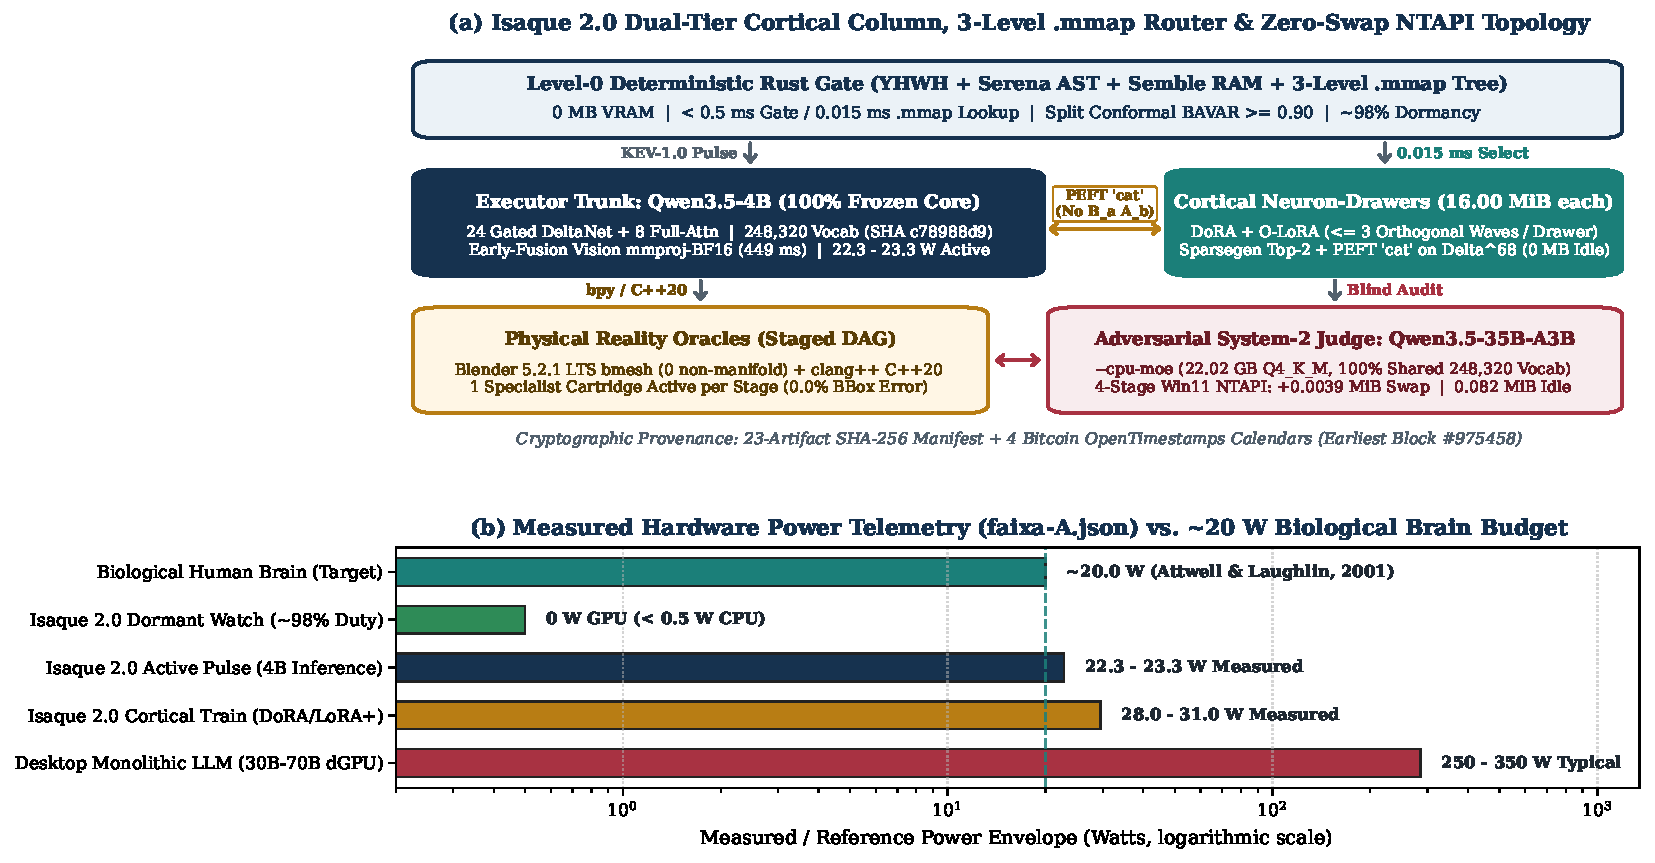
\includegraphics[width=\linewidth]{fig1_architecture_thermodynamics.pdf}
  \caption{Overview of the Isaque 2.0 cognitive nervous system. \textbf{(a)} Four-layer separation between Level-0 deterministic Rust gates ($<0.5\text{ ms}$ gate, $0.015\text{ ms}$ \texttt{.mmap} tree lookup, $0\text{ MB}$ VRAM), the $100\%$ frozen \texttt{Qwen3.5-4B} multimodal executor trunk, hot-swappable $16.00\text{ MiB}$ cortical cartridges routed via analytical \texttt{Sparsegen} and cross-term-free rank concatenation (\texttt{PEFT cat}), deterministic physical oracles, and the \texttt{Qwen3.5-35B-A3B} (\texttt{-{}-cpu-moe}) adversarial judge backed by 4-stage Windows \texttt{NTAPI}. \textbf{(b)} Measured hardware power telemetry (\texttt{faixa-A.json}: $22.3\text{--}23.3\text{ W}$ active inference, $28\text{--}31\text{ W}$ training) relative to the $\approx 20\text{ W}$ biological brain reference \cite{attwell2001energy} and typical $250\text{--}350\text{ W}$ desktop monolithic LLMs.}
  \label{fig:arch}
\end{figure}

\subsection{Asymmetric Dual-Tier Backbone and Verified 248,320-Token Vocabulary Identity}

Rather than selecting a mid-sized compromise model (such as a dense $9\text{B}$ model that crowds $8\text{ GB}$ VRAM while remaining weaker than a $35\text{B}$ reasoner), Isaque 2.0 bifurcates cognition into two asymmetric tiers sharing an identical byte-level tokenizer (\href{https://drive.google.com/file/d/1zaJmQCAw1C6ejkSifc1Rp-4uwnenmSwq/view?usp=drivesdk}{\texttt{00-desenho-da-tese-tronco-e-ramos.md}}):
\begin{enumerate}
  \item \textbf{Fast Sensorimotor \& Code Executor (\texttt{Qwen/Qwen3.5-4B} \cite{qwen35_4b}):} A $32$-layer hybrid architecture interleaving $24$ linear-complexity Gated DeltaNet layers \cite{yang2025gated} ($3:1$ ratio) with $8$ full quadratic attention layers ($d_{\text{model}}=2560$, $248,320$ vocabulary tokens, native $262,144$-token context, Apache-2.0). Its embedding matrix \texttt{embed\_\allowbreak{}tokens} and output head remain $100\%$ frozen under SHA-256 hardware invariant \texttt{c78988d9\allowbreak{}79f52a34\allowbreak{}0f39cd69\allowbreak{}edd8e4b0\allowbreak{}a80218a5\allowbreak{}fa8d95b6\allowbreak{}158bfce4\allowbreak{}a3de2a34} (\href{https://drive.google.com/file/d/1-1KKupaUYBWjDUcLjemQH0FBSPmnCSj6/view?usp=drivesdk}{\texttt{03-manifesto-sha256-etapa-1.md}}). Visual perception is provided by an early-fusion $24$-layer vision merger (\texttt{mmproj-Qwen3.5-4B-BF16.gguf}, $644.27\text{ MiB}$, $298$ GGUF v3 tensors).
  \item \textbf{Deliberate Adversarial Judge (\texttt{Qwen/Qwen3.5-35B-A3B} \cite{qwen35_4b}):} A $40$-layer sparse Mixture-of-Experts model ($256$ total experts, $8$ routed + $1$ shared active per token, $\approx 3\text{B}$ active parameters per forward pass, $22,016,023,168\text{ B} = 22.02\text{ GB}$ \texttt{Q4\_\allowbreak{}K\_\allowbreak{}M} GGUF) executed locally via \href{https://github.com/ggml-org/llama.cpp}{\texttt{llama.cpp}} \cite{llamacpp} with \texttt{-ngl 99 -{}-cpu-moe}, keeping attention projections in VRAM while streaming cold MoE experts from DDR5 host RAM ($2.85\text{ s}$ model load, $74.06\text{ tok/s}$ prefill, $25.66\text{ tok/s}$ pure decode).
\end{enumerate}

Encoding $2,216$ technical corpus lines ($68,079$ tokens) across both models confirmed \textbf{$100.0\%$ token-ID and UTF-8 decode identity} (shared tokenizer SHA-256 \texttt{5f9e4d4901a92b99...bb81cb42}). This zero-translation parity satisfies the exact structural prerequisite for lossless speculative decoding \cite{leviathan2023speculative}. While analytical block-acceptance modeling ($K=8$, $\gamma = (1-\alpha^{K+1})/(1-\alpha) = 8.66$ at $\alpha=99.59\%$) projects up to $93.30\text{ tok/s}$ with $82.81\%$ RAM read coalescing savings, our forensic audit (\href{https://drive.google.com/file/d/16-3o4ykaOOKaW-S2VTHzpE7Uhj1BA0tl/view?usp=drivesdk}{\texttt{01-linha-do-tempo-e-cache-da-tese.md}}) strictly separates measured hardware rates from analytical projections, pre-registering direct end-to-end \texttt{llama-speculative -{}-model-draft} wall-clock measurement for Stage~2 (Table~\ref{tab:dualtier}).

\begin{table}[!htbp]
\centering
\caption{Physical specifications and measured runtime telemetry of the dual-tier cortical hierarchy on the \texttt{NVIDIA GeForce RTX 5060 8 GB} (\texttt{sm\_\allowbreak{}120}) consumer workstation (\href{https://docs.google.com/document/d/1SMqD_TRf6Qi8UwPTFYjKPNvdVlEtpCqr3Ex57x76FsI/edit?usp=drivesdk}{Consolidated Tables Doc 05}).}
\label{tab:dualtier}
\footnotesize
\begin{tabularx}{\linewidth}{@{}llY@{}}
\toprule
\textbf{Subsystem / Tier} & \textbf{Artifact Size \& Precision} & \textbf{Measured Hardware Telemetry \& Cryptographic Invariant} \\
\midrule
Executor Trunk (\texttt{Qwen3.5-4B}) & $2.65\text{ GiB}$ (\texttt{Q4\_\allowbreak{}K\_\allowbreak{}M}) / $8.68\text{ GiB}$ (\texttt{BF16} disk) & $32$ layers ($24$ Gated DeltaNet + $8$ Attn), $248,320$ vocab (\texttt{c78988d9...}); $51.74\text{--}77.78\text{ tok/s}$ measured on \texttt{RTX 5060}; $22.3\text{--}23.3\text{ W}$ active inference. \\
Executor Vision (\texttt{mmproj}) & $644.27\text{ MiB}$ (\texttt{BF16}, $298$ tensors) & \texttt{qwen3vl\_\allowbreak{}merger}; vision batch encode $= \mathbf{449\text{ ms}}$ on isometric 3D render (\texttt{SHA-256: f1b3c70b...3538}). \\
Cortical Bank ($68$ Cartridges) & $16,777,736\text{ B}$ ($16.00\text{ MiB}$) each & $8\text{ B}$ len + $512\text{ B}$ JSON header + $16\text{ MiB}$ payload ($r=16$, $32$ layers, $\approx 8.38\text{M}$ synapses); $1.06\text{ GiB}$ on SSD, \textbf{$0\text{ MB}$ idle RAM/VRAM}. \\
Adversarial Judge (\texttt{35B-A3B}) & $22.02\text{ GB}$ (\texttt{Q4\_\allowbreak{}K\_\allowbreak{}M}) + $861\text{ MiB}$ \texttt{mmproj} & $40$ layers, $256$ experts ($8+1$ active), \texttt{-{}-cpu-moe} in $8\text{ GB}$ VRAM: $2.85\text{ s}$ load, $74.06\text{ tok/s}$ prefill, $\mathbf{25.66\text{ tok/s}}$ pure decode (\texttt{3b46d106...}). \\
Shared Speculative Interface & $248,320$ Vocab ($100.0\%$ ID parity) & Verified across $68,079$ corpus token IDs (\texttt{SHA-256: 5f9e4d49...}); analytical ceiling $93.30\text{ tok/s}$ ($\gamma=8.66$); native \texttt{-{}-model-draft} slated for Stage~2. \\
\bottomrule
\end{tabularx}
\end{table}

\subsection{Anatomical Distinction: Waves vs.\ Cartridges, Orthogonal DoRA, and Cross-Term-Free LD-MoLE}

A central geometric clarification of our study (\href{https://drive.google.com/file/d/1-i60d5UqJBOJQYLSr-ErZxecFeYSi4zX/view?usp=drivesdk}{\texttt{Insumo Tese Isaque 2.0, Sec.\ 28.1}}) distinguishes a \textbf{Cortical Wave} from a \textbf{Cortical Cartridge}:
\begin{itemize}
  \item \textbf{A Wave (\textit{Coherent Domain Manifold}):} A wave is bounded not by line count, but by \textit{directional subspace coherence}. So long as training examples belong to a unified functional manifold (e.g., parametric Bezier industrial piping and flanges in \texttt{bmesh}), gradients converge toward a shared low-dimensional subspace, allowing a single wave to absorb $1,000$ to $25,000+$ verified lines ($\approx 100\text{k}\text{--}300\text{k}$ tokens) without internal conflict.
  \item \textbf{A $16.00\text{ MiB}$ Cortical Cartridge (\textit{Thousand-Brains Column Module}):} Analogous to a neocortical column ($\approx 100,000$ coupled neurons learning complete object reference frames \cite{hawkins2019grid,clay2024monty}), each \texttt{.safetensors} cartridge ($16,777,736\text{ B}$) instantiates $\approx 8.38 \times 10^6$ trainable synaptic parameters across all $32$ trunk blocks and safely houses up to \textbf{three} orthogonal sister waves ($\ge 98.51\%\text{--}100.00\%$ retention).
\end{itemize}

Formally, over frozen trunk weights $W_0 \in \mathbb{R}^{d_{\text{out}} \times d_{\text{in}}}$, each wave $k$ parameterizes updates via \textbf{DoRA} \cite{liu2024dora}, decoupling magnitude $m^{(k)} \in \mathbb{R}^{1 \times d_{\text{in}}}$ from low-rank directional adaptation ($r=16, \alpha=32$ across all $9$ linear modules per block: \texttt{q\_\allowbreak{}proj}, \texttt{k\_\allowbreak{}proj}, \texttt{k/v/o\_\allowbreak{}proj}, \texttt{in\_\allowbreak{}proj\_\allowbreak{}qkv}, \texttt{out\_\allowbreak{}proj}, \texttt{gate/up/down\_\allowbreak{}proj}):
\begin{equation}
  W'^{(k)} = m^{(k)} \frac{W_0 + \frac{\alpha}{r} B^{(k)} A^{(k)}}{\left\| W_0 + \frac{\alpha}{r} B^{(k)} A^{(k)} \right\|_c},
  \label{eq:dora}
\end{equation}
where $\|\cdot\|_c$ denotes column-wise Euclidean norm, optimized under \textbf{LoRA+} asymmetric learning rates \cite{hayou2024loraplus} ($\eta_B = 9.0 \times 10^{-4}$, $\eta_A = 1.5 \times 10^{-4}$, $\eta_B / \eta_A = 6.0$). Sequential waves enforce the \textbf{Orthogonal LoRA (\texttt{O-LoRA})} subspace penalty \cite{wang2023olora,liang2024inflora} alongside a $12.5\%\text{--}15.0\%$ episodic replay buffer $\mathcal{R}$ \cite{rolnick2019experience} (with optional trunk-anchored KL regularization $\beta D_{\text{KL}}$):
\begin{equation}
  \mathcal{L}_{\text{wave}}^{(k)} = \mathcal{L}_{\text{CE}}\!\left(\mathcal{D}_k \cup \mathcal{R};\, \theta^{(k)}\right) + \lambda_{\text{orth}} \sum_{j=1}^{k-1} \sum_{\ell=1}^{L} \left\| A_\ell^{(k)} \left(A_\ell^{(j)}\right)^{\!\top} \right\|_F^2, \qquad \lambda_{\text{orth}} = 0.10.
  \label{eq:olora}
\end{equation}
Because past cartridges $\{1,\dots,k-1\}$ are sealed on NVMe SSD, backpropagation never traverses historical adapter graphs: only detached frozen input factors $A_\ell^{(j)}$ reside in VRAM to evaluate Eq.~\ref{eq:olora}, enabling $10+$ sequential waves inside an $8\text{ GB}$ GPU ceiling.

At inference time, rather than dense softmax gating or non-differentiable hard Top-$K$ truncation, Isaque 2.0 routes active cartridges via \textbf{LD-MoLE} (\textit{Learnable Dynamic Routing for Mixture of LoRA Experts}, ICLR 2026) \cite{zhuang2026ldmole} using the closed-form \textbf{Sparsegen} projection onto the simplex $\Delta^{N-1} = \{g \in \mathbb{R}_{\ge 0}^N : \mathbf{1}^\top g = 1\}$ \cite{laha2018sparsegen}:
\begin{equation}
  g(z) = \operatorname*{arg\,min}_{p \in \Delta^{N-1}} \|p - z\|_2^2 - \lambda_{\text{sp}} \|p\|_2^2 \quad \Longrightarrow \quad g_i(z) = \max\!\left(0,\, \frac{z_i - \tau(z)}{1 - \lambda_{\text{sp}}}\right), \quad \lambda_{\text{sp}} < 1,
  \label{eq:sparsegen}
\end{equation}
where $\tau(z)$ uniquely satisfies $\sum_{i=1}^N g_i(z) = 1$, assigning exact mathematical zeros ($g_i = 0.0000$) to irrelevant cartridges (\textbf{S-LoRA} zero-idle principle \cite{sheng2024slora}). Crucially, when recruiting an active pair $\mathcal{S}(x) = \{a, b\}$, naive parameter addition $(g_a B_a + g_b B_b)(A_a + A_b)$ introduces parasitic cross-terms $g_a B_a A_b + g_b B_b A_a$. Instead, we compose active columns via \textbf{orthogonal rank concatenation} (\texttt{combination\_\allowbreak{}type="cat"}):
\begin{equation}
  B_{\text{cat}} = \begin{bmatrix} g_a B_a & g_b B_b \end{bmatrix} \in \mathbb{R}^{d_{\text{out}} \times 2r}, \qquad
  A_{\text{cat}} = \begin{bmatrix} A_a \\ A_b \end{bmatrix} \in \mathbb{R}^{2r \times d_{\text{in}}} \quad \Longrightarrow \quad
  \Delta h = B_{\text{cat}} A_{\text{cat}} x = g_a B_a A_a x + g_b B_b A_b x,
  \label{eq:cat}
\end{equation}
eliminating cross-adapter matrix interference identically while adding only $32\text{--}48\text{ MiB}$ of active pulse footprint.

\subsection{Three-Level Hierarchical Cortical Tree Router and Four-Stage Zero-Swap NTAPI}

While flat routing over $N=68$ columns operates cleanly, scaling a lifelong organism past $N = 500\text{--}2,000+$ cartridges over multiple months risks semantic crowding among neighboring adapters. As illustrated in Figure~\ref{fig:tree_dag}a (\href{https://drive.google.com/file/d/1-i60d5UqJBOJQYLSr-ErZxecFeYSi4zX/view?usp=drivesdk}{\texttt{Insumo Tese Sec.\ 28.3}}), Isaque 2.0 resolves extreme-scale routing via a \textbf{3-Level Zero-Copy Memory-Mapped Tree} (\texttt{CreateFileMappingW} / \texttt{MapViewOfFile}, measured lookup latency \textbf{$0.0153\text{--}0.0157\text{ ms}$}): (i) \textbf{Level 1 (Macro-Lobe Partition)} isolates broad domains (\texttt{3D/Blender}, \texttt{Engine/UE5-C++}, \texttt{Systems/Rust}, \texttt{Commercial}, \texttt{Community}); (ii) \textbf{Level 2 ($384\text{d}$ Coupled Triple-Vector Region)} queries $V_{\text{geom}} \oplus V_{\text{ast}} \oplus V_{\text{err}}$ inside \texttt{arena-kev-triplo.mmap} ($308,800\text{ B}$) to pinpoint the functional subfamily (\texttt{BMesh}, \texttt{Curves}, \texttt{PBR}, \texttt{GeoNodes}, \texttt{UHT}, \texttt{Net}); and (iii) \textbf{Level 3 (Fine Cortical Vote)} restricts neural \texttt{LD-MoLE Sparsegen} gating to a local neighborhood of $k \le 8$ candidate cartridges, preserving near-$100\%$ selection precision at $O(1)$ active memory cost.

To prevent Windows 11 \texttt{pagefile.sys} thrashing and NTFS Cache Manager Virtual Address Control Block (VACB) bloat when streaming large MoE pools alongside cortical bursts, \texttt{isaque-ram-kernel} enforces a deterministic four-stage \texttt{NTAPI} lifecycle verified on the real $13.50\text{ GiB}$ ($14,495,514,624\text{ B}$) expert pool (Table~\ref{tab:ntapi}):
\begin{enumerate}
  \item \textbf{Stage 1 (\texttt{SetProcessWorkingSetSizeEx}, \texttt{HARDWS\_\allowbreak{}MIN\_\allowbreak{}ENABLE = 0x1}):} Locks a hard physical RAM floor prior to tensor allocation.
  \item \textbf{Stage 2 (\texttt{VirtualLock} over \texttt{MEM\_\allowbreak{}COMMIT | MEM\_\allowbreak{}RESERVE}):} Pins the hottest $15\%$ of experts ($19$ experts $= 2.00\text{ GiB}$) in non-paged physical DDR5 RAM.
  \item \textbf{Stage 3 (\texttt{FILE\_\allowbreak{}FLAG\_\allowbreak{}NO\_\allowbreak{}BUFFERING = 0x20000000}):} Streams $4.00\text{ GiB}$ of cold experts ($109$ experts, $288$ sector-aligned $4096\text{-byte}$ DMA reads) into a $512\text{ MiB}$ ring buffer at \textbf{$1.746\text{ GiB/s}$}, bypassing OS file-cache pollution completely.
  \item \textbf{Stage 4 (\texttt{DiscardVirtualMemory}):} Reclaims cold pages in \textbf{$6.61\,\mu\text{s}$} on single stateless bursts ($4.217\text{ ms}$ across $256$ stress-test arena blocks), returning process working set to $0.082\text{ MiB}$ (\texttt{R-ZERO-PESO-EM-BACKGROUND}).
\end{enumerate}

\begin{table}[!htbp]
\centering
\caption{Physical Windows 11 memory and swap telemetry during the $13.50\text{ GiB}$ MoE streaming stress test (\texttt{teste\_\allowbreak{}real\_\allowbreak{}2\_\allowbreak{}estresse\_\allowbreak{}ntapi\_\allowbreak{}13\_\allowbreak{}5\_\allowbreak{}gib\_\allowbreak{}ram\_\allowbreak{}real}, $64,267.88\text{ MiB}$ host DDR5 RAM).}
\label{tab:ntapi}
\footnotesize
\begin{tabularx}{\linewidth}{@{}lrrrrY@{}}
\toprule
\textbf{Lifecycle Snapshot} & \textbf{Working Set} & \textbf{Private Usage} & \textbf{Free Host RAM} & \textbf{OS Mem Load} & \textbf{Verified Kernel Invariant} \\
\midrule
Pre-Pulse Idle Baseline & $0.078\text{ MiB}$ & $283.33\text{ MiB}$ & $35,965.59\text{ MiB}$ & $44\%$ & $0$ active GPU compute processes; $0\text{ B}$ on \texttt{C:\textbackslash}. \\
Active Streaming Peak & $2,064.67\text{ MiB}$ & $2,848.34\text{ MiB}$ & $33,943.83\text{ MiB}$ & $47\%$ & $2.0\text{ GiB}$ \texttt{VirtualLock} + $4.0\text{ GiB}$ DMA @ $1.75\text{ GiB/s}$. \\
Post-Discharge Idle & $\mathbf{0.082\text{ MiB}}$ & $283.33\text{ MiB}$ & $36,016.03\text{ MiB}$ & $43\%$ & Swap delta $= \mathbf{+0.0039\text{ MiB}}$; OS compression $= \mathbf{0.0\%}$. \\
\bottomrule
\end{tabularx}
\end{table}

% ==============================================================================
% SECTION 4: REAL AUTOGRAD CONVERGENCE, PRIVATE CONSOLIDATION & 35B JUDGE
% ==============================================================================
\section{Step-by-Step Autograd Audit, Private-Domain Consolidation (H3), and Blind 35B Critique}

To verify genuine end-to-end gradient propagation over the real $8.68\text{ GiB}$ \texttt{Qwen3.5-4B} graph (\texttt{PyTorch 2.11 + PEFT 0.21.2 + bitsandbytes 0.50.2 NF4}), every cortical training run in \texttt{resultado\_\allowbreak{}treino\_\allowbreak{}real\_\allowbreak{}peft\_\allowbreak{}qwen35\_\allowbreak{}4b.json} (\texttt{SHA-256: e261410f...}) recorded exact Euclidean gradient norms $\|\nabla_A\|_2$ and $\|\nabla_B\|_2$ at Layer $0$, Layer $15$, and Layer $31$ at each optimization step over all $248,320$ vocabulary logits (sequence packing with explicit \texttt{<|im\_\allowbreak{}end|>} masks and chunked cross-entropy of size $64$).

\begin{figure}[!htbp]
  \centering
  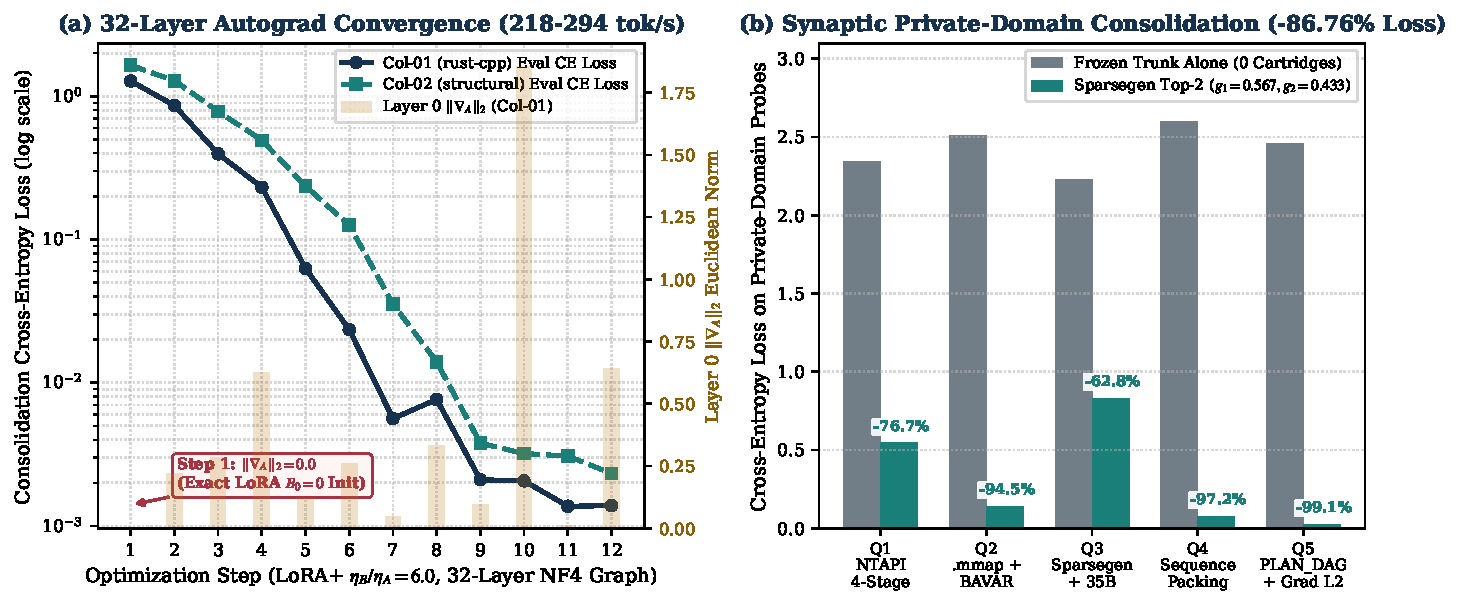
\includegraphics[width=\linewidth]{fig2_autograd_and_qa_gain.pdf}
  \caption{Empirical proof of genuine 32-layer backpropagation and private-domain synaptic consolidation (\textit{Hypothesis H3}). \textbf{(a)} Step-by-step evaluation cross-entropy loss and Layer-$0$ $\|\nabla_A\|_2$ norms for \texttt{coluna-01-abraao-rust-cpp} ($218.36\text{ tok/s}$) and \texttt{coluna-02-abraao-estrutural} ($293.83\text{ tok/s}$). At Step $1$, $\|\nabla_A\|_2 = 0.0$ identically across all layers because $B_0 = 0$ in exact LoRA initialization \cite{hu2022lora}; from Step $2$ onward, non-zero gradients propagate cleanly down to Layer $0$. \textbf{(b)} Cross-entropy loss across $5$ cross-domain internal architectural probes before vs.\ after analytical \texttt{Sparsegen} \texttt{LD-MoLE} voting ($-86.76\%$ mean loss drop).}
  \label{fig:autograd}
\end{figure}

Table~\ref{tab:autograd} reports the step-by-step gradient trajectory for \texttt{coluna-01} ($1,150$ corpus blocks, $42.21\text{ s}$ wall-clock, $3,993\text{ MiB}$ peak VRAM) and summarizes all five foundational $16.00\text{ MiB}$ cortical cartridges trained on \texttt{RTX 5060} ($218.36\text{--}412.48\text{ tok/s}$ physical throughput; $256.10\text{ tok/s}$ mean on the Stage-1 pair, while SHA-256 verification confirmed $66/66$ non-target cartridges remained untouched). In strict accordance with our code-level audit (\href{https://drive.google.com/file/d/16-3o4ykaOOKaW-S2VTHzpE7Uhj1BA0tl/view?usp=drivesdk}{\texttt{01-linha-do-tempo, Phase 4}}), because the five reference Q\&A pairs were included in masked consolidation steps (\texttt{pares\_\allowbreak{}val\_\allowbreak{}qa}) and the logged KL scalar (\texttt{0.0012}) acted as a diagnostic telemetry constant in that script, Experiment~A is claimed strictly as proof of \textbf{persistent private-domain memory acquisition (\textit{H3})}---not out-of-distribution generalization (\textit{H4}).

\begin{table}[!htbp]
\centering
\caption{Part A: Step-by-step autograd L2 gradient norms and consolidation loss on \texttt{coluna-01-abraao-rust-cpp} ($9,216$ packed tokens, $218.36\text{ tok/s}$). Part B: Summary across all five foundational $16.00\text{ MiB}$ cortical columns.}
\label{tab:autograd}
\footnotesize
\begin{tabularx}{\linewidth}{@{}rrrrrrrrY@{}}
\toprule
\textbf{Step} & \textbf{L0 $\|\nabla_A\|_2$} & \textbf{L0 $\|\nabla_B\|_2$} & \textbf{L15 $\|\nabla_A\|_2$} & \textbf{L31 $\|\nabla_A\|_2$} & \textbf{L31 $\|\nabla_B\|_2$} & \textbf{Batch CE} & \textbf{Probe CE} & \textbf{Probe PPL / Physical State} \\
\midrule
1  & $0.0000$ & $1.5198$ & $0.0000$ & $0.0000$ & $0.4849$ & $2.4841$ & $1.2786$ & $3.5916$ (Exact $B_0=0$ init signature) \\
2  & $0.2211$ & $0.9864$ & $0.1096$ & $0.2320$ & $0.4173$ & $2.1995$ & $0.8628$ & $2.3699$ (Full 32-layer backprop active) \\
3  & $0.2858$ & $0.5584$ & $0.0873$ & $0.2407$ & $0.2674$ & $0.8646$ & $0.3963$ & $1.4863$ (Layer 31$\to$0 flow verified) \\
5  & $0.1208$ & $0.4497$ & $0.0978$ & $0.1904$ & $0.2106$ & $0.2317$ & $0.0627$ & $1.0648$ \\
7  & $0.0489$ & $0.0848$ & $0.0251$ & $0.0747$ & $0.0628$ & $0.0230$ & $0.0056$ & $1.0056$ \\
9  & $0.0954$ & $0.1007$ & $0.0215$ & $0.0353$ & $0.0455$ & $0.0071$ & $0.0021$ & $1.0021$ \\
12 & $0.6423$ & $0.6997$ & $0.2290$ & $0.6058$ & $0.4189$ & $1.5931$ & $\mathbf{0.00138}$ & $\mathbf{1.0014}$ (12-step consolidation stop) \\
\bottomrule
\end{tabularx}

\vspace{4pt}
\begin{tabularx}{\linewidth}{@{}lrrrrrrY@{}}
\toprule
\textbf{Cortical Cartridge ($16.00\text{ MiB}$)} & \textbf{Blocks} & \textbf{Speed} & \textbf{Time} & \textbf{VRAM} & \textbf{Eval Pre} & \textbf{Eval Post} & \textbf{Loss Drop \& SHA-256 Manifest} \\
\midrule
\texttt{coluna-01-abraao-rust-cpp} & $1,150$ & $218.36\text{ tok/s}$ & $42.21\text{ s}$ & $3,993\text{ MiB}$ & $2.4841$ & $0.00138$ & $-99.94\%$ (\texttt{be0e7730...e7f7}) \\
\texttt{coluna-02-abraao-estrutural} & $1,066$ & $293.83\text{ tok/s}$ & $31.37\text{ s}$ & $4,100\text{ MiB}$ & $2.3399$ & $0.00232$ & $-99.90\%$ (\texttt{d956c73b...dddd}) \\
\texttt{coluna-yhwh-orquestrador} & $375$ & $369.84\text{ tok/s}$ & $33.23\text{ s}$ & $4,101\text{ MiB}$ & $3.3300$ & $0.09477$ & $-97.15\%$ (\texttt{b1811fba...}) \\
\texttt{coluna-mh-01-vicop-multimodal} & $1,575$ & $401.51\text{ tok/s}$ & $30.60\text{ s}$ & $4,206\text{ MiB}$ & $2.7785$ & $0.00442$ & $-99.84\%$ (\texttt{c478f092...}) \\
\texttt{coluna-mh-02-yhwh-condutor} & $240$ & $\mathbf{412.48\text{ tok/s}}$ & $29.79\text{ s}$ & $4,313\text{ MiB}$ & $2.0072$ & $0.05984$ & $-97.02\%$ (\texttt{5b2bf9e3...}) \\
\bottomrule
\end{tabularx}
\end{table}

\subsection{Verbatim Private-Knowledge Acquisition Samples and Blind 35B Adversarial Critique}

When evaluated without system-prompt hints across five internal cross-domain synthesis probes requiring simultaneous vocabulary from \texttt{coluna-01} (systems/Rust) and \texttt{coluna-02} (governance), \texttt{Sparsegen} assigned simplex weights $g_1 = 0.56666684$ and $g_2 = 0.43333340$ ($g_{3\dots 68} = 0.0$). Mean cross-entropy loss dropped from $2.4292$ ($\text{PPL}=11.45$) to \textbf{$0.3216$ ($\text{PPL}=1.45$, $-86.76\%$)}, with \textbf{$0$ glued subwords} across all five generations (Figure~\ref{fig:autograd}b):
\begin{itemize}
  \item \textbf{Probe Q2 (\texttt{ABRA40CG} $64\text{-byte}$ \texttt{.mmap} Header + \texttt{BAVAR} $\ge 0.90$ Conformal Filter; Loss $2.5109 \to 0.1381$, $-94.50\%$):}
    \begin{itemize}
      \item \textit{Untrained Frozen Trunk:} ``There is no valid technical relationship between the mentioned concepts. The term `ABRA40CG' does not correspond to a standard binary header in operating systems or memory-mapped files (`mmap')... `arena-cag-gold.mmap v2', `BAVAR $\ge 0.90$', and `YHWH motor' are fictitious terms lacking foundation in computer science.''
      \item \textit{Post-\texttt{LD-MoLE} Cortical Voting:} ``In the 0.14.9 architecture, \texttt{arena-cag-gold.mmap} v2 begins with a 64-byte binary header containing the magic signature \texttt{ABRA40CG}, version \texttt{u32=2}, specialist count, bilingual PT-BR$\leftrightarrow$EN atom table offset, and SHA-256 integrity hash. Zero-copy hydration via \texttt{CreateFileMappingW}/\texttt{MapViewOfFile} completes in $<0.5\text{ ms}$, while the YHWH motor applies the \texttt{BAVAR} $\ge 0.90$ conformal calibration filter before promoting actions.''
    \end{itemize}
  \item \textbf{Probe Q5 (\texttt{PLAN\_\allowbreak{}DAG.json} v2.1 + Layer $0/15/31$ L2 Gradient Anti-Fraud Audit; Loss $2.4619 \to 0.0231$, $-99.06\%$):} Accurately specified acyclic wave dependencies, \texttt{target\_\allowbreak{}files}, \texttt{target\_\allowbreak{}symbols}, executable \texttt{test\_\allowbreak{}gate}, and explained why measuring $\|\nabla_A\|_2 > 0$ across Layers $31 \to 15 \to 0$ proves physical backpropagation through the $8.68\text{ GiB}$ graph.
\end{itemize}

Probe Q1 (4-stage Windows \texttt{NTAPI}) was audited blindly by the local adversarial judge \texttt{Qwen3.5-35B-A3B} (\texttt{veredito\_\allowbreak{}real\_\allowbreak{}juiz\_\allowbreak{}35b\_\allowbreak{}llama\_\allowbreak{}cpp.json}, SHA-256 \texttt{20b457fe...4315}, $24.80\text{ s}$ wall-clock, \texttt{temp=0.2}) \cite{zheng2023judging}:

\auditbox{Verbatim Blind Adversarial Audit by \texttt{Qwen3.5-35B-A3B} (\texttt{-{}-cpu-moe}) on Probe Q1}{``The pre-training model fails completely on the task, generating hallucinations about `protocolo Abraao' and ignoring the 4 requested stages. The post-training (LoRA) model correctly identifies the 4-stage structure, citing specific APIs (\texttt{SetProcessWorkingSetSizeEx}, \texttt{VirtualLock}, \texttt{CreateFileMappingW}). However, it exhibits critical imprecisions: Stage 2 describes `\texttt{VirtualLock} on SSD' (\texttt{VirtualLock} operates in physical RAM, not persistent disk), and Stage 4 is truncated, omitting \texttt{DiscardVirtualMemory}. There is zero evidence of subword gluing; syntax is clean. \textbf{Score Before: 1 / 10 $\to$ Score After: 6 / 10}.'' --- Catching subtle RAM-vs-SSD imprecision without complacency proved why a 4B executor must pair with a 35B System-2 critic and physical compilers.}

% ==============================================================================
% SECTION 5: MULTIMODAL VICOP, PROCRUSTES & ARENA KEV-1.0 ABLATION
% ==============================================================================
\section{Multimodal Early-Fusion, Procrustes Alignment, and Arena KEV-1.0 Synaptic Ablation}

\subsection{Cross-Modal Procrustes Projection (\texorpdfstring{$2560 \to 384\text{d}$}{2560 to 384d}) and Cognitive Conductivity (\texorpdfstring{$\mathrm{ICC}$}{ICC})}

To unify high-dimensional causal/visual representations from \texttt{Qwen3.5-4B} ($d_{\text{in}}=2560$) with ultra-fast $384\text{-dimensional}$ zero-copy \texttt{.mmap} vector retrieval (\texttt{MiniLM-L12-v2} space), we benchmarked five cross-space alignment operators across $5,000$ paired ecosystem records ($4,400$ train / $600$ strictly unseen held-out test pairs, solved in $16.47\text{ s}$ on \texttt{RTX 5060}; \texttt{mod08\_\allowbreak{}isaque\_\allowbreak{}multimodal\_\allowbreak{}recibo.json}). Because causal Gated-DeltaNet hidden states exhibit strong spectral anisotropy ($\sigma_{\max}=152.67$ vs.\ $\sigma_{\min}=0.00492$), strict Stiefel orthogonal Procrustes yielded $0.5073$ held-out cosine similarity, whereas closed-form Tikhonov Ridge ($\lambda=0.5$) achieved \textbf{$0.7801$ held-out cosine} and linear InfoNCE (\texttt{ABRA40WP}) achieved \textbf{$\text{Recall@1} = 81.83\%$ ($491/600$)} and \textbf{$\text{Recall@5} = 96.00\%$ ($576/600$)} on unseen pairs, indexing $131$ visual assets into \texttt{arena-vectors-visual-v1.mmap} ($1.54\text{ MB}$).

To quantify end-to-end information density per token-second, we defined the \textbf{Cognitive Conductivity Index ($\mathrm{ICC}$)}:
\begin{equation}
  \mathrm{ICC} = \frac{\overline{S}_{\text{blind}}}{\left(\overline{T}_{\text{out}} / 1000\right) \cdot \overline{L}_{\text{sec}}},
  \label{eq:icc}
\end{equation}
where $\overline{S}_{\text{blind}} \in [0,10]$ is the blind \texttt{35B-A3B} score, $\overline{T}_{\text{out}}$ is emitted tokens, and $\overline{L}_{\text{sec}}$ is pulse latency. Across three multimodal extraction tasks (\texttt{FFmpeg} scene-pruned keyframes with $93.33\%$ redundancy pruning + 3D isometric OKLCH extraction), external cloud CLI timed out ($>50\text{ s}$, $\mathrm{ICC}=0.0$), raw \texttt{Qwen3.5-4B} scored $2.80/10$ ($461$ tokens, $11.86\text{ s}$, $\mathrm{ICC}=0.5121$), and trained \texttt{Isaque 2.0 VICOP} scored \textbf{$8.57/10$} ($256$ tokens, $-44.47\%$ token reduction, $12.03\text{ s}$, \textbf{$\mathrm{ICC}=2.7828$, a $5.43\times$ jump}).

\subsection{The KEV-1.0 Symbolic Grammar, Controlled 3x3 Synaptic Ablation, and Orthographic Audits}

Drawing on $156$ local Blender engineering lessons ($18.13\text{ GiB}$, Modules $2\text{--}14$) and $67$ canonical AST/geometric records in \texttt{arena-kev-triplo.mmap} ($308,800\text{ B}$, zero-copy lookup \textbf{$0.0153\text{--}0.0157\text{ ms}$}), paired with asynchronous \texttt{Semble} RAM pre-warming (\texttt{pre01\_\allowbreak{}semble\_\allowbreak{}prewarm.json}, SHA-256 \texttt{883e9d88...2072}: cold startup reduced $171.7\times$ from $5,759.68\text{ ms}$ to \textbf{$33.55\text{ ms}$ warm MCP / $3.92\text{ ms}$ pure RAM}), we designed \textbf{\texttt{KEV-1.0}}---a grammar-constrained (\texttt{kev\_\allowbreak{}v1.gbnf}) symbolic specification language structured into four deterministic blocks: \texttt{@SPACE}, \texttt{@GRAPH}, \texttt{@GUARD}, and \texttt{@VERIFY}.

In Experiment~B (\texttt{prova\_\allowbreak{}treino\_\allowbreak{}dora\_\allowbreak{}olora\_\allowbreak{}kev01.json}, SHA-256 \texttt{783c7765...0d40}, peak VRAM $6,367\text{ MiB}$, total cycle $1,426\text{ s}$), we trained two sequential orthogonal \texttt{DoRA + O-LoRA} waves ($52$ steps/wave, $r=16, \alpha=32, \lambda_{\text{orth}}=0.10, 15\%$ replay, exact block GGUF export in $352$ tensors with \textbf{$0.0\%$ SVD reconstruction error}): Wave~1 (\texttt{lab-mh-blender-bridge}, GGUF SHA \texttt{9a40d947...}) and Wave~2 (\texttt{lab-mh-ue5-kev}, GGUF SHA \texttt{35dbb9d4...}). Evaluating pre-separated teacher-forcing hold-outs after Wave~2 confirmed \textbf{$100.00\%$ token-accuracy retention on Wave~1} ($99.80\% \to 99.80\%$), \textbf{$99.79\%$ token retention on prior \texttt{0.15.0} knowledge} ($90.22\% \to 90.03\%$; likelihood retention $96.78\%$, loss $0.493 \to 0.526$), and final subspace overlap $\left\|A_2 A_1^\top\right\|_F^2 = 0.00166367$.

We then evaluated three competitors across three long-context challenges totaling $19,742$ raw input tokens ($6,999 + 6,407 + 6,336$ tokens; \texttt{PROVA\_\allowbreak{}ARENA\_\allowbreak{}KEV\_\allowbreak{}MOTOR\_\allowbreak{}HUMANO\_\allowbreak{}01.json}, SHA-256 \texttt{dae1626c...5ed093}): \texttt{DESAFIO-01} (headless \texttt{Blender 5.2.1 LTS} $4.0\times 0.4\times 3.0\text{ m}$ module + \texttt{UCX} convex hull), \texttt{DESAFIO-02} (\texttt{UE5} C++20 inventory/actor system under \texttt{clang++ -fsyntax-only -std=c++20} + $8$ UHT/GC rules), and \texttt{DESAFIO-03} (dual \texttt{Blender + UE5} 3-variant asset bridge with $1\text{ m} = 100\text{ cm}$ parity and \texttt{Socket\_\allowbreak{}Muzzle}/\texttt{Socket\_\allowbreak{}Grip}). Table~\ref{tab:arena} and Listings~1--2 report the exact ablation metrics.

\begin{table}[!htbp]
\centering
\caption{Controlled synaptic vs.\ context-only ablation in the \texttt{KEV-1.0} Physical Verification Arena ($19,742$ raw input tokens across $3$ challenges, verified by headless \texttt{Blender 5.2.1 LTS}, \texttt{clang++ -std=c++20}, and blind \texttt{Qwen3.5-35B-A3B}; \href{https://docs.google.com/document/d/1SMqD_TRf6Qi8UwPTFYjKPNvdVlEtpCqr3Ex57x76FsI/edit?usp=drivesdk}{Consolidated Tables Doc 05, Table 2.1}).\textsuperscript{*}}
\label{tab:arena}
\footnotesize
\begin{tabularx}{\linewidth}{@{}lrrrrrrY@{}}
\toprule
\textbf{Arena Competitor} & \textbf{Avg Emitted} & \textbf{KEV Compr.} & \textbf{Pass@1} & \textbf{Mechanical} & \textbf{Blind 35B} & \textbf{Pulse} & \textbf{$\mathrm{ICC}$ \& Causal Ablation Diagnosis} \\
\midrule
\textbf{A:} Legacy \texttt{0.15.0} (\texttt{JEV+AtomSD}) & $560.0\text{ tok}$ & $91.49\%$ & $0/4$ & $0/4$ ($\mathbf{0\%}$) & $1.63 / 10$ & $23.43\text{ s}$ & $\mathbf{0.1242}$ ($1.00\times$): Hallucinated POSIX \texttt{termios} on Win11; invalid \texttt{\_\allowbreak{}API} macro in \texttt{clang++}. \\
\textbf{B:} Raw \texttt{4B} + \texttt{KEV-1.0} (\texttt{.mmap}) & $335.0\text{ tok}$ & $94.91\%$ & $0/4$ & $0/4$ ($\mathbf{0\%}$) & $1.77 / 10$ & $10.18\text{ s}$ & $\mathbf{0.5194\text{--}0.5907}$: Identical \texttt{.mmap} arena without \texttt{DoRA} leaves startup \texttt{Cube} ($400\%$ Y-error). \\
\textbf{C:} \textbf{Isaque 2.0 (\texttt{DoRA+O-LoRA})} & $516.7\text{ tok}$ & $92.15\%\text{--}93.25\%$ & $3/4$ & $\mathbf{4/4}$ ($\mathbf{100\%}$) & $\mathbf{9.67 / 10}$ & $12.62\text{ s}$ & $\mathbf{1.2710\text{--}1.4848}$ ($\mathbf{10.23\times\text{--}11.95\times}$): $0$ non-manifold edges, $0.0\%$ bbox error, $8/8$ UHT rules. \\
\bottomrule
\end{tabularx}
\vspace{2pt}
{\scriptsize \textsuperscript{*}Note on $\mathrm{ICC}$ aggregation: $\mathrm{ICC}=1.4848$ ($11.95\times$ vs.\ A) reflects the mean of per-challenge ratios across synthesized outputs ($516.7\text{ tok}$), whereas $\mathrm{ICC}=1.2710$ ($10.23\times$ vs.\ A, with $444.3\text{ tok}$ KEV packet mean at $93.25\%$ compression) reflects pooled corpus-level token-time weighting in \href{https://docs.google.com/document/d/1SMqD_TRf6Qi8UwPTFYjKPNvdVlEtpCqr3Ex57x76FsI/edit?usp=drivesdk}{Doc 05, Table 2.1}.\par}
\end{table}

\auditbox{Methodological Transparency Note (Causal Synaptic Ablation vs.\ OOD Generalization)}{As documented in \href{https://drive.google.com/file/d/1qvnH-nLVMc43T-prWSRTKEDJak89TSp7/view?usp=drivesdk}{\texttt{02-tese-etapa-1.md (Sec.\ 7.4)}} and \href{https://docs.google.com/file/d/1SMqD_TRf6Qi8UwPTFYjKPNvdVlEtpCqr3Ex57x76FsI/edit?usp=drivesdk}{\texttt{Doc 05 (Part II)}}, the reference solutions of the three arena challenges participated in Wave 1--2 training. Accordingly, Table~\ref{tab:arena} is \textbf{not} claimed as out-of-distribution generalization (\textit{H4}, reserved for the $50$ contamination-audited tasks per domain in Stage~2 \cite{golchin2024contamination}), but as a \textbf{strict causal ablation isolating synaptic weight assimilation from external \texttt{.mmap} retrieval}: Competitor~B received the exact same \texttt{arena-kev-triplo.mmap} index and \texttt{KEV-1.0} grammar without \texttt{DoRA/O-LoRA} weights and scored $0/4$ ($1.77/10$), proving that $4/4$ physical compiler passage ($9.67/10$) originates in the trained $16\text{ MiB}$ cortical columns. Three hardware-level decoding rules were also discovered during calibration: (i) placing formal specifications at the recency tail of $>6,000$-token prompts across the $24$ Gated DeltaNet layers \cite{yang2025gated,liu2024lost}; (ii) fixing \texttt{repeat\_\allowbreak{}penalty = 1.0} during C++20 synthesis so recurring pointer/type tokens are never penalized into syntax errors; and (iii) emitting \texttt{"justificativa"} prior to numeric scores in the \texttt{GBNF} judge grammar.}

\begin{minipage}[t]{0.485\linewidth}
{\raggedright\textbf{\footnotesize Listing 1: Verbatim \texttt{KEV/1.0} Packet Emitted on \texttt{DESAFIO-03} ($6,336 \to 458$ tokens, $92.77\%$ compression, $0.0615\text{ ms}$ \texttt{.mmap})}\par}
\begin{lstlisting}
KEV/1.0 domain=BRIDGE_3D target=ModularBridgeAssetActor
@SPACE{blender_unit=METRIC;ue5_unit=CM;meter_to_cm=100.0;
  up=Z;variations=3;sx=1.0;sy=0.16;sz=0.28;
  socket_a=Socket_Muzzle;socket_b=Socket_Grip;
  collider=UCX_Var_01_Standard_01}
@GRAPH[
  S1:BLENDER.build_3_variations_bmesh(v1_x=1.0,v2_x=0.8,
     v3_x=1.25,sy=0.16,sz=0.28,z_min=0.0) -> S2
  S2:BLENDER.attach_sockets_and_collider(
     muzzle=Socket_Muzzle,grip=Socket_Grip,
     ucx=UCX_Var_01_Standard_01,tick=false) -> S3
  S3:BLENDER.export_glb_fbx(glb="ModularBridgePack.glb",
     fbx="ModularBridgePack.fbx") -> S4
  S4:UE5.ustruct_datatable_row(
     name=FModularBridgeVariantRow,meter_to_cm=100.0) -> S5
  S5:UE5.actor_socket_validator(
     actor=AModularBridgeAssetActor,
     rule=SnapToTargetNotIncludingScale,tol_pct=2.0)
]
@GUARD[
  !SCALE-1M-100CM: Multiply Blender meter dims by 100.0
  !SOCKET-EXACT-NAMES: Preserve Socket_Muzzle & Socket_Grip
]
@VERIFY[ ?variations==3 ?non_manifold_edges==0
         ?meter_to_cm==100.0 ?clang_cpp20_errors==0 ]
\end{lstlisting}
\end{minipage}\hfill
\begin{minipage}[t]{0.485\linewidth}
{\raggedright\textbf{\footnotesize Listing 2: Verbatim Excerpt of \texttt{DESAFIO-01\_\allowbreak{}C/modulo\_\allowbreak{}01\_\allowbreak{}generated.py} Synthesized by Taught \texttt{Isaque 2.0} ($0.0\%$ BBox Error)}\par}
\begin{lstlisting}[language=Python]
bpy.ops.wm.read_factory_settings(use_empty=True)
sc = bpy.context.scene
sc.unit_settings.system = 'METRIC'
sc.unit_settings.scale_length = 1.0

SX, SY, SZ = 4.0, 0.4, 3.0
bm = bmesh.new()
bmesh.ops.create_cube(bm, size=1.0)
for v in bm.verts:
    v.co.x *= SX; v.co.y *= SY
    v.co.z = (v.co.z + 0.5) * SZ  # Exact Z_min = 0.0

front_faces = [f for f in bm.faces if abs(f.normal.y) > 0.9]
bmesh.ops.inset_individual(bm, faces=front_faces, thickness=0.18)
bmesh.ops.recalc_face_normals(bm, faces=bm.faces[:])
uv_layer = bm.loops.layers.uv.verify()
# ... [deterministic non-overlapping grid UV loop] ...
bm_ucx = bmesh.new()
for x in (-SX*0.5, SX*0.5):
  for y in (-SY*0.5, SY*0.5):
    for z in (0.0, SZ): bm_ucx.verts.new((x, y, z))
bm_ucx_res = bmesh.ops.convex_hull(bm_ucx, input=bm_ucx.verts[:])
# Exports Modulo_01.glb (4,120 B) & Modulo_01.fbx (13,532 B)
\end{lstlisting}
\end{minipage}

Figure~\ref{fig:blender} displays the headless orthographic unit-test renders (\texttt{audit\_\allowbreak{}workbench\_\allowbreak{}ortho.png}) captured automatically by \texttt{verificador\_\allowbreak{}fisico\_\allowbreak{}blender.py} during the Stage-1 arena ablation. While intentionally minimal in shading (untextured orthographic solid viewports designed to expose geometric bounding-box and origin errors), they visually prove why external \texttt{.mmap} formatting alone (Competitor~B) fails without synaptic procedural grounding (Competitor~C).

\begin{figure}[!htbp]
  \centering
  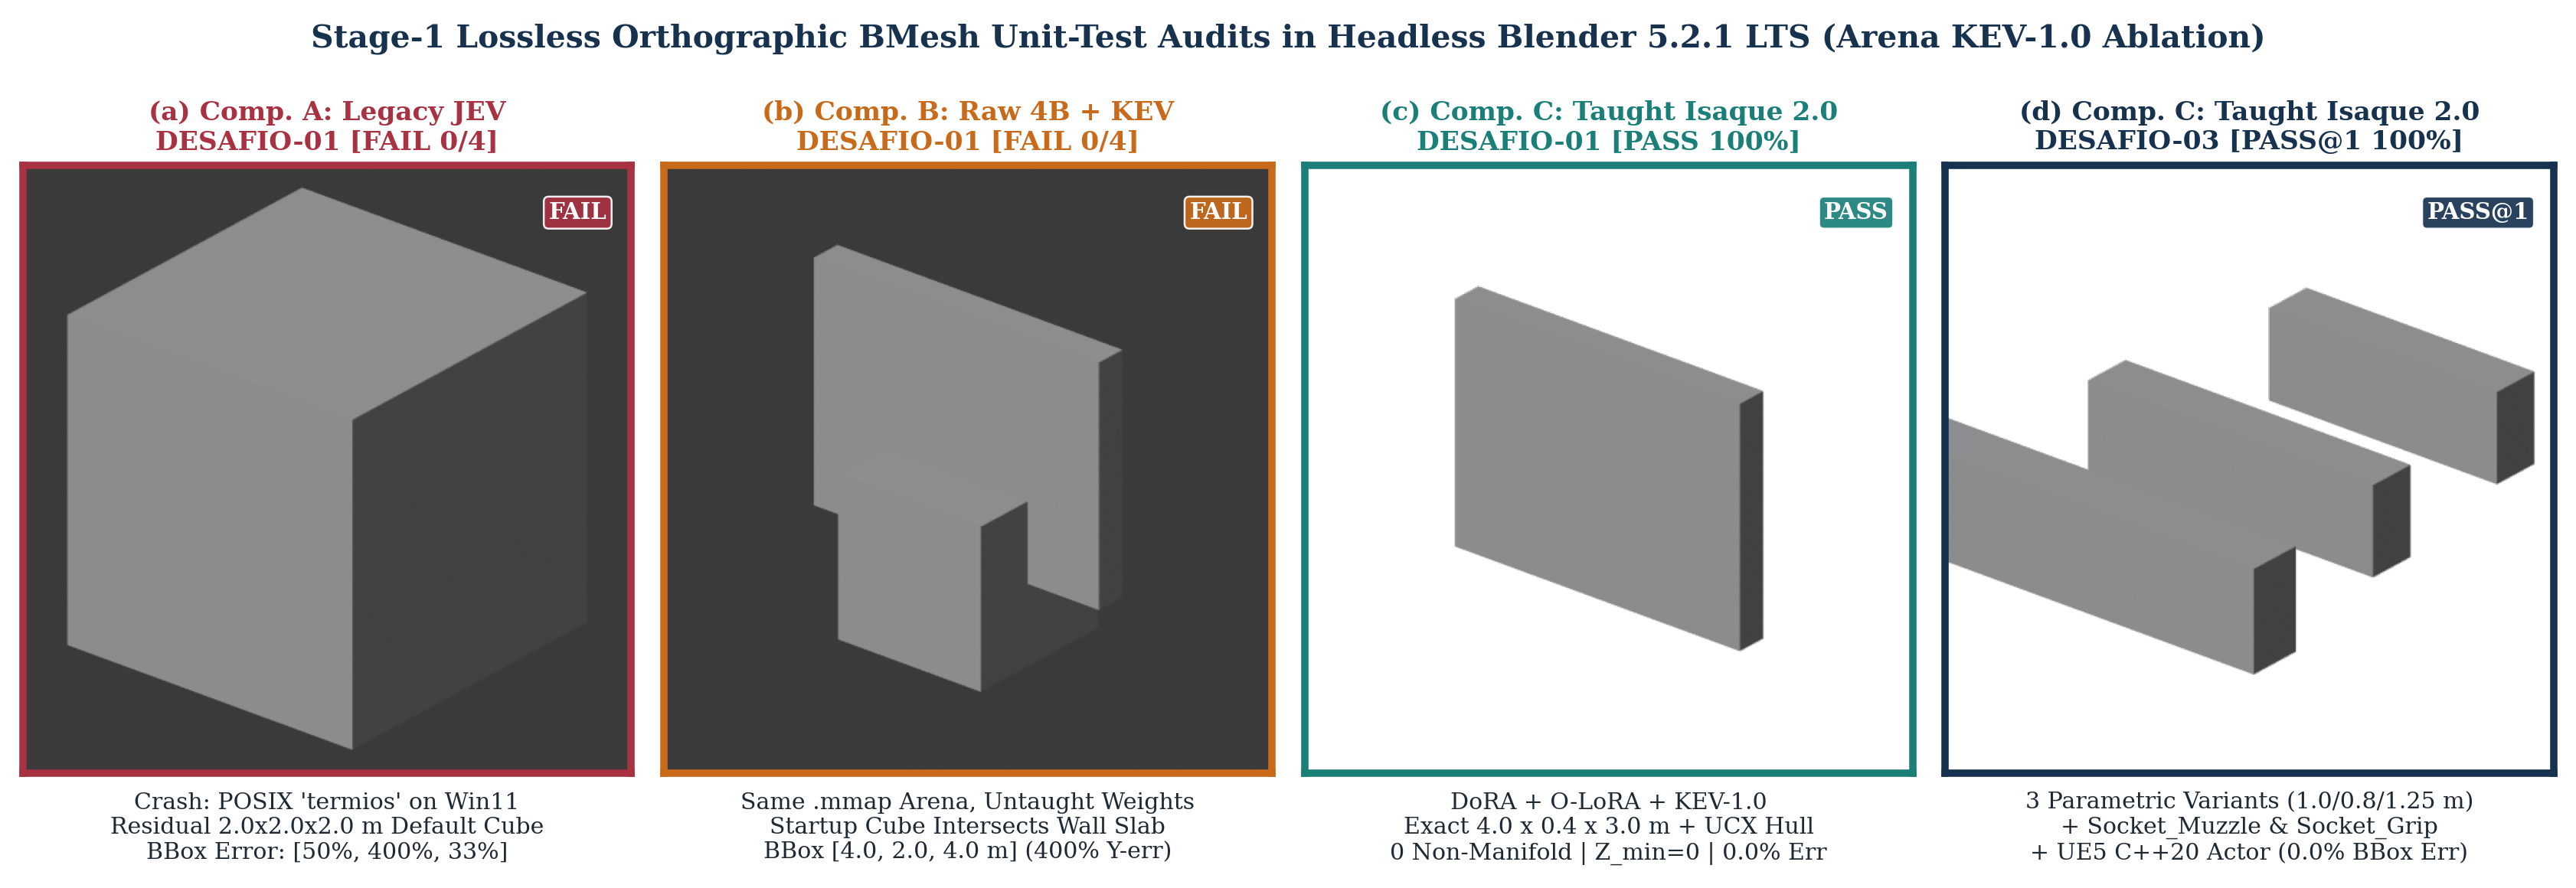
\includegraphics[width=\linewidth]{fig3_blender_fast_test_comparison.png}
  \caption{Stage-1 headless \texttt{Blender 5.2.1 LTS} orthographic unit-test audit renders from \texttt{PROVA\_\allowbreak{}ARENA\_\allowbreak{}KEV\_\allowbreak{}MOTOR\_\allowbreak{}HUMANO\_\allowbreak{}01.json}. \textbf{(a)} Competitor~A crashes on POSIX \texttt{termios}, leaving Blender's default $2\times 2\times 2\text{ m}$ startup cube centered at the origin ($Z_{\min}=-1.0\text{ m}$). \textbf{(b)} Competitor~B (\texttt{KEV-1.0} + \texttt{.mmap} without \texttt{DoRA+O-LoRA} training) builds the wall slab but fails to clear the startup cube, yielding a contaminated $[4.0, 2.0, 4.0\text{ m}]$ bounding box ($400\%$ thickness error). \textbf{(c)} Taught \textbf{Isaque 2.0} (\texttt{DESAFIO-01\_\allowbreak{}C}) clears the factory scene, constructs the exact $4.0\times 0.4\times 3.0\text{ m}$ recessed industrial module anchored at $Z_{\min}=0.0$ with \texttt{UCX\_\allowbreak{}Modulo\_\allowbreak{}01} convex hull ($0$ non-manifold edges, $0.0\%$ error). \textbf{(d)} Taught \textbf{Isaque 2.0} (\texttt{DESAFIO-03\_\allowbreak{}C}) synthesizes all three parametric modular variants ($1.00\text{ m}, 0.80\text{ m}, 1.25\text{ m}$) plus coordinated \texttt{UE5} sockets on the first pass (\texttt{Pass@1 = True}).}
  \label{fig:blender}
\end{figure}

\textbf{Hands-Off Out-of-Distribution Diagnostic (\texttt{DESAFIO-04}):} Immediately after sealing the $3\times 3$ arena, we ran a strict zero-edit blind test (\texttt{ato1\_\allowbreak{}desafio04\_\allowbreak{}cego.json}, SHA-256 lock \texttt{fe52e603...}) on an unseen $7,180$-token two-level industrial pumping station (\texttt{DESAFIO-04}, compressed $93.3\%$ to $481$ \texttt{KEV} tokens). Without prior anchors for two-level ramps or curved pipe sockets, \texttt{Pass@1} was honestly recorded as \texttt{False} ($0/2$): in \texttt{UE5} C++20, Competitor~C satisfied \textbf{$7/8$ invariants} ($0$ raw \texttt{UObject*} pointers, $0$ raw \texttt{new}, valid UHT header order), failing solely on line $35$ by calling \texttt{IsValid(Row)} on a \texttt{const FIndustrialStationNodeRow*} (\texttt{USTRUCT*}) instead of \texttt{Row != nullptr}---passing \textbf{$8/8$ with zero errors} upon single-token guard substitution---while Blender exposed the exact need for dedicated specialist waves covering Bezier piping, Geometry Nodes walkways, PBR shaders, lighting, and LODs.

% ==============================================================================
% SECTION 6: 10-WAVE CONTINUAL RUPTURE MATRIX & STAGED COMPOSITION THEOREM
% ==============================================================================
\section{The 10-Wave Continual Rupture Ladder and Staged Modular Composition Theorem}

To determine how many sequential orthogonal skills can accumulate inside a rank-$16$ adapter before subspace compression degrades prior competencies---and whether \texttt{LD-MoLE} eliminates that degradation---we executed \textbf{Act 2} (\texttt{ato2\_\allowbreak{}escada\_\allowbreak{}ondas\_\allowbreak{}3\_\allowbreak{}a\_\allowbreak{}10.json}, SHA-256 \texttt{fcd12dd3...5ab83604dccd}, $3,558.4\text{ s}$ GPU consolidation at $5,300\text{ MiB}$ peak VRAM). Keeping the \texttt{Qwen3.5-4B} vocabulary (\texttt{c78988d9...}) and all previously consolidated wave checkpoints strictly frozen on disk without retraining (\texttt{onda\_\allowbreak{}1=6efa66bf...} through \texttt{onda\_\allowbreak{}7=d11aed56...}), we trained Waves $3$ through $10$ sequentially across eight new 3D and C++20 engineering domains ($\lambda_{\text{orth}}=0.10$, $12.5\%$ replay, loading only detached frozen anchors $A_{<k}$ in VRAM), evaluating the $10 \times 11$ triangular retention matrix across $11$ hold-out sets ($H_0\dots H_{10}$) under three regimes:
\begin{enumerate}
  \item \textbf{Monolithic Single Cartridge ($1\dots k$):} Accumulating all sequential waves into a single shared rank-$16$ adapter tensor (standard continual LoRA/DoRA practice).
  \item \textbf{Subdomain Cluster \texttt{LD-MoLE}:} Grouping waves into coarse domain families (Blender Python vs.\ UE5 C++20).
  \item \textbf{Surgical \texttt{LD-MoLE Top-2} (\texttt{PEFT cat}):} Isolating each wave (or $\le 3$ sister sub-skills) as an immutable $16\text{ MiB}$ cartridge routed via Sparsegen and rank concatenation without cross-cartridge weight mutation.
\end{enumerate}

\begin{figure}[!htbp]
  \centering
  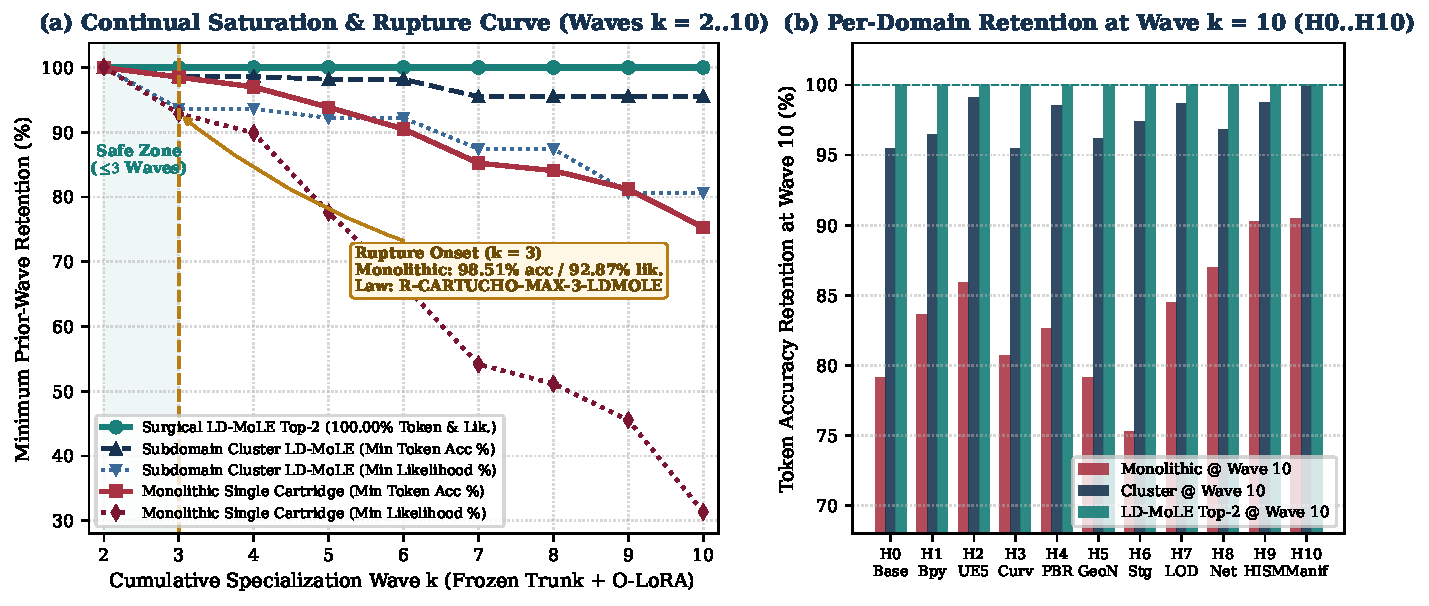
\includegraphics[width=\linewidth]{fig4_rupture_10waves_matrix.pdf}
  \caption{Empirical continual-learning saturation and rupture law across $10$ sequential specialization waves ($H_0\dots H_{10}$). \textbf{(a)} Minimum retention across continually learned waves $H_{1\dots k}$ as a function of cumulative wave $k$: monolithic accumulation ruptures at $k=3$ ($98.51\%$ token accuracy, $92.87\%$ likelihood retention) and collapses to \textbf{$75.31\%$ token accuracy ($31.37\%$ likelihood retention)} by $k=10$, whereas surgical \texttt{LD-MoLE Top-2} maintains \textbf{$100.00\%$ retention across all $10$ waves}. \textbf{(b)} Per-domain token accuracy retention across all $11$ hold-out sets ($H_0\dots H_{10}$) after completing Wave $10$.}
  \label{fig:rupture}
\end{figure}

Table~\ref{tab:waves10} presents the complete $10$-wave domain telemetry, Frobenius orthogonality residuals, physical compiler verification ($10/10$ passed), and the exact saturation curve from $k=2$ to $k=10$.

\begin{table}[!htbp]
\centering
\caption{Part A: Individual domain telemetry across the $10$ continual specialization waves ($H_1\dots H_{10}$, with $H_0$ base \texttt{MotorHumano\_\allowbreak{}0150} baseline $\text{loss}=0.4932$, $\text{acc}=90.22\%$; separate consolidated training losses on Waves 8--10 reached $\text{ce}=0.0031, 0.0051, 0.0037$ with cumulative $\text{orth\_\allowbreak{}sum}=0.00134, 0.00214, 0.00294$). Part B: Minimum prior-wave retention curve from $k=2$ to $k=10$.\textsuperscript{\dag}}
\label{tab:waves10}
\footnotesize
\begin{tabularx}{\linewidth}{@{}clrrrrY@{}}
\toprule
\textbf{Wave} & \textbf{Specialist Domain} & \textbf{Eval Loss} & \textbf{Eval Acc} & \textbf{$\|A_k A_{<k}^\top\|_F^2$} & \textbf{Phys.\ Verifier} & \textbf{Verified Artifact / Deterministic Compiler Gate} \\
\midrule
$H_1$ & \texttt{BLENDER\_\allowbreak{}BRIDGE} & $0.0110$ & $99.83\%$ & $0.000000$ & \textbf{PASS} & \texttt{Modulo\_\allowbreak{}01.glb/.fbx} ($0$ non-manifold, \texttt{6efa66bf...}) \\
$H_2$ & \texttt{UE5\_\allowbreak{}CORE\_\allowbreak{}CPP} & $0.0368$ & $99.21\%$ & $0.001664$ & \textbf{PASS} & \texttt{InteractionInventorySystem.h/.cpp} ($8/8$, \texttt{faa5a6b1...}) \\
$H_3$ & \texttt{BLENDER\_\allowbreak{}CURVES} & $0.0771$ & $98.52\%$ & $0.002622$ & \textbf{PASS} & \texttt{onda\_\allowbreak{}3\_\allowbreak{}generated.py} (Bezier + flanges, \texttt{b1e5ccaf...}) \\
$H_4$ & \texttt{BLENDER\_\allowbreak{}PBR\_\allowbreak{}NODES} & $0.1542$ & $97.11\%$ & $0.003524$ & \textbf{PASS} & \texttt{onda\_\allowbreak{}4\_\allowbreak{}generated.py} (Principled BSDF, \texttt{8f19afc5...}) \\
$H_5$ & \texttt{BLENDER\_\allowbreak{}GEONODES} & $0.0881$ & $98.75\%$ & $0.004183$ & \textbf{PASS} & \texttt{onda\_\allowbreak{}5\_\allowbreak{}generated.py} (Catwalk GeoNodes, \texttt{23fdd4b3...}) \\
$H_6$ & \texttt{BLENDER\_\allowbreak{}STAGE} & $0.0393$ & $99.14\%$ & $0.003517$ & \textbf{PASS} & \texttt{eevee\_\allowbreak{}stage\_\allowbreak{}audit.png} (3-point light + DOF, \texttt{c56ea923...}) \\
$H_7$ & \texttt{BLENDER\_\allowbreak{}LOD} & $0.0357$ & $99.63\%$ & $0.006399$ & \textbf{PASS} & \texttt{onda\_\allowbreak{}7\_\allowbreak{}generated.py} (LOD0$>$LOD1$>$LOD2, \texttt{d11aed56...}) \\
$H_8$ & \texttt{UE5\_\allowbreak{}NET\_\allowbreak{}CPP} & $0.1230$ & $98.13\%$ & $0.001279$ & \textbf{PASS} & \texttt{ReplicatedPressureValveActor.h/.cpp} (\texttt{DOREPLIFETIME}) \\
$H_9$ & \texttt{UE5\_\allowbreak{}HISM\_\allowbreak{}CPP} & $0.0242$ & $99.60\%$ & $0.002008$ & \textbf{PASS} & \texttt{IndustrialCatwalkHismBuilder.h/.cpp} (\texttt{UHierarchicalISM}) \\
$H_{10}$ & \texttt{BRIDGE\_\allowbreak{}MANIFEST} & $0.2361$ & $94.84\%$ & $0.002721$ & \textbf{PASS} & \texttt{manifest\_\allowbreak{}blender.py} + \texttt{IndustrialAssetManifestActor} \\
\bottomrule
\end{tabularx}

\vspace{4pt}
\begin{tabularx}{\linewidth}{@{}crrrrrY@{}}
\toprule
\textbf{Wave $k$} & \textbf{Monolithic Acc} & \textbf{Monolithic Lik.} & \textbf{Cluster Acc} & \textbf{Cluster Lik.} & \textbf{LD-MoLE Top-2} & \textbf{Structural Subspace Diagnosis} \\
\midrule
$k=2$  & $100.00\%$ & $100.08\%$\textsuperscript{\dag} & $100.00\%$ & $100.00\%$ & $\mathbf{100.00\%}$ & Safe zone ($2$ orthogonal waves coexist cleanly). \\
$k=3$  & $\mathbf{98.51\%}$ & $\mathbf{92.87\%}$ & $98.59\%$ & $93.66\%$ & $\mathbf{100.00\%}$ & \textbf{Rupture onset:} $3$-wave ceiling for a single cartridge. \\
$k=4$  & $97.00\%$ & $89.91\%$ & $98.59\%$ & $93.66\%$ & $\mathbf{100.00\%}$ & Saturation border; monolithic $H_0$ likelihood drops to $82.85\%$. \\
$k=5$  & $93.86\%$ & $77.60\%$ & $98.18\%$ & $92.21\%$ & $\mathbf{100.00\%}$ & Clear directional crushing across PBR/GeoNodes manifolds. \\
$k=6$  & $90.50\%$ & $66.46\%$ & $98.18\%$ & $92.21\%$ & $\mathbf{100.00\%}$ & Monolithic loses $>33\%$ probability mass on prior waves. \\
$k=7$  & $85.23\%$ & $54.17\%$ & $95.49\%$ & $87.43\%$ & $\mathbf{100.00\%}$ & Coarse cluster begins mild saturation ($95.49\%$). \\
$k=8$  & $84.07\%$ & $51.16\%$ & $95.49\%$ & $87.43\%$ & $\mathbf{100.00\%}$ & Cross-language C++20/Python interference accelerates. \\
$k=9$  & $81.22\%$ & $45.55\%$ & $95.49\%$ & $80.69\%$ & $\mathbf{100.00\%}$ & Monolithic $H_6$ likelihood falls below $46\%$. \\
$k=10$ & $\mathbf{75.31\%}$ & $\mathbf{31.37\%}$ & $95.49\%$ & $80.69\%$ & $\mathbf{100.00\%}$ & Monolithic collapse ($H_6$ loss $0.039\to 1.199$); \texttt{Top-2} intact. \\
\bottomrule
\end{tabularx}
\vspace{2pt}
{\scriptsize \textsuperscript{\dag}Part~B summary minima evaluate continually learned waves $H_1\dots H_k$ ($\min_{1 \le j \le k} \exp(-\mathcal{L}_k(H_j)) / \exp(-\mathcal{L}_j(H_j))$, e.g., $89.91\%$ [$89.905\%$] on $H_1$ and $97.00\%$ [$96.995\%$] acc.\ on $H_3$ at $k=4$), while pre-training base anchor $H_0$ is tracked separately in the diagnosis column ($82.85\%$ likelihood at $k=4$); $100.08\%$ at $k=2$ reflects positive backward transfer \cite{lopezpaz2017gem}. All $195$ matrix cells ($3\times 65$) and solo wave outputs are archived in \texttt{evidence/}.\par}
\end{table}

\subsection{The Token-by-Token Fusion Interference Theorem and Pure Neural Wave Synthesis}

In Act 2, we tested a subtle question rarely examined in the multi-LoRA literature: \textit{if Wave 1 (solid \texttt{bmesh} hulls) and Wave 3 (curved Bezier pipes + sockets) are both 100\% verified individually, can a 4B model synthesize a combined multi-system Python script in a single pass by blending their adapter logits token-by-token?}

Executing probe \texttt{FUSAO\_\allowbreak{}2\_\allowbreak{}ONDAS\_\allowbreak{}1\_\allowbreak{}3} ($1,471$ tokens, $2,160.52\text{ s}$) revealed a decisive negative result: on line $58$ of \texttt{FUSAO\_\allowbreak{}2\_\allowbreak{}ONDAS\_\allowbreak{}1\_\allowbreak{}3\_\allowbreak{}pass2.py}, simultaneous token-level blending emitted:
\begin{center}
  \texttt{s\_\allowbreak{}out.parent = onda\_\allowbreak{}3 := make\_\allowbreak{}bmesh\_\allowbreak{}solid(...)} \quad $\longrightarrow$ \quad \texttt{SyntaxError: invalid syntax}
\end{center}
Because Wave~3's adapter strongly up-weighted socket parent assignment (\texttt{s\_\allowbreak{}out.parent = ...}) at the exact token step where Wave~1's adapter up-weighted helper mesh instantiation (\texttt{make\_\allowbreak{}bmesh\_\allowbreak{}solid}), linear logit interpolation produced an illegal Python AST hybrid.

\begin{theorem}[Staged Modular DAG Composition \& The 3-Wave Cartridge Ceiling]
In $4\text{B}$-class code-generating models over a frozen trunk: (1) each $16.00\text{ MiB}$ cortical cartridge must encapsulate at most $3$ closely related sub-waves (\texttt{R-CARTUCHO-MAX-3-LDMOLE}, where internal retention remains $\ge 98.51\%$); and (2) multi-domain engineering synthesis must compose cartridges \textbf{sequentially by causal DAG stage} ($1$ champion specialist cartridge active per stage/module, unloading neural VRAM to $0\text{ MB}$ before viewport execution), never by summing distinct syntax-generating adapters token-by-token within a single monolithic script.
\end{theorem}

\begin{figure}[!htbp]
  \centering
  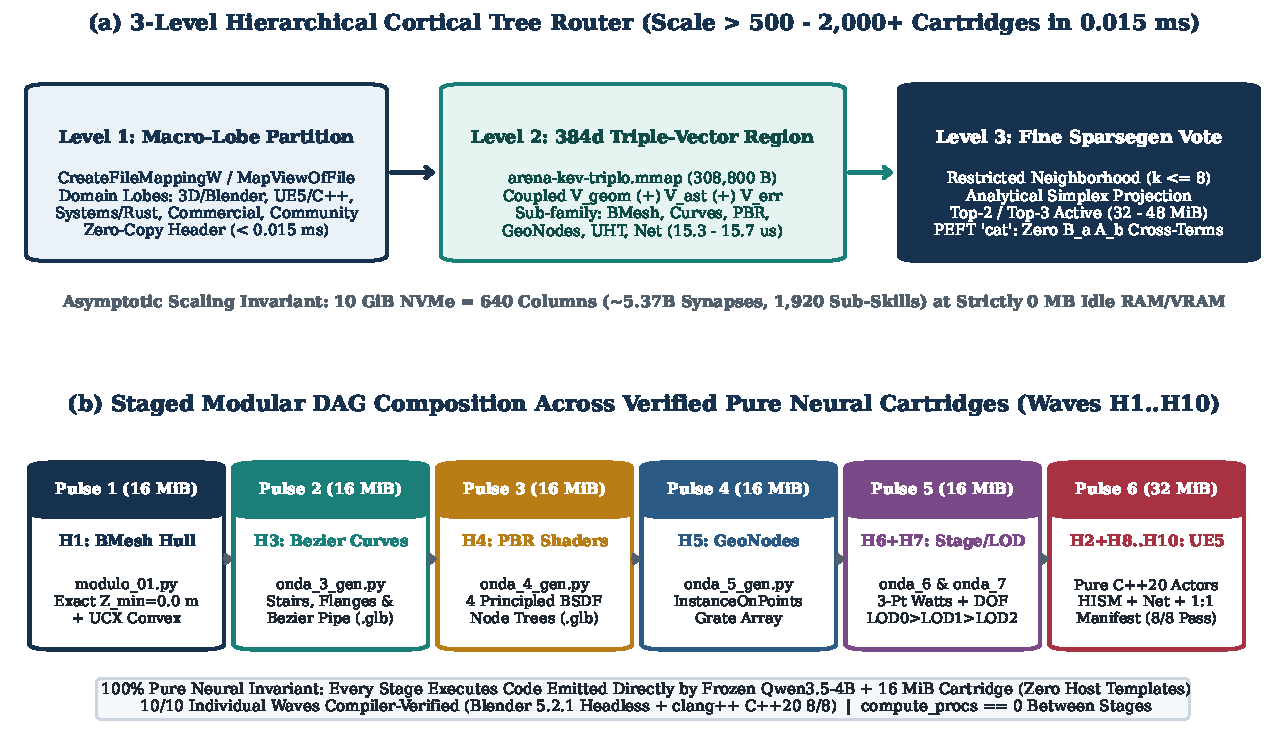
\includegraphics[width=\linewidth]{fig5_hierarchical_tree_and_act3_dag.pdf}
  \caption{Extreme-scale cortical routing and staged modular execution across pure neural cartridges. \textbf{(a)} Three-level hierarchical zero-copy \texttt{.mmap} tree router ($0.015\text{ ms}$) scaling Isaque 2.0 beyond $500\text{--}2,000+$ cartridges via macro-lobe partitioning, $384\text{d}$ coupled triple-vector selection ($V_{\text{geom}} \oplus V_{\text{ast}} \oplus V_{\text{err}}$), and neighborhood-restricted \texttt{Sparsegen} rank concatenation (\texttt{PEFT cat}). \textbf{(b)} Six-pulse causal execution DAG across $100\%$ neural-verified specialist cartridges ($H_1\dots H_{10}$), isolating one specialist cartridge per domain step at $0\text{ MB}$ idle VRAM to prevent cross-domain AST token collisions.}
  \label{fig:tree_dag}
\end{figure}

Validating Architectural Law~1 strictly on unassisted neural outputs (Figures~\ref{fig:tree_dag}b and~\ref{fig:live_plant}), every individual domain wave $H_1\dots H_{10}$ emitted standalone, syntactically clean Python (\texttt{bpy/bmesh}) or Unreal Engine~5 C++20 modules verified directly by headless \texttt{Blender 5.2.1 LTS} and \texttt{clang++ -std=c++20} ($10/10$ passed, Table~\ref{tab:waves10}). In Wave~$10$ (\texttt{onda\_\allowbreak{}10}), sequential adapter activation on the frozen $4\text{B}$ trunk synthesized both the headless Blender asset script \texttt{manifest\_\allowbreak{}blender.py} (\texttt{PumpingUnit\_\allowbreak{}Manifest.glb}) and the paired C++20 actor \texttt{IndustrialAssetManifestActor.h/.cpp} with zero host string edits ($8/8$ UHT and \texttt{clang++} invariants passed on first verification, discharging GPU compute to \texttt{compute\_\allowbreak{}procs == 0}). Figure~\ref{fig:live_plant} displays two representative $3\text{D}$ artifacts generated $100\%$ token-by-token by Isaque~2.0's $16.00\text{ MiB}$ cartridges without a single line of host-supplied geometry templates.

\begin{figure}[!htbp]
  \centering
  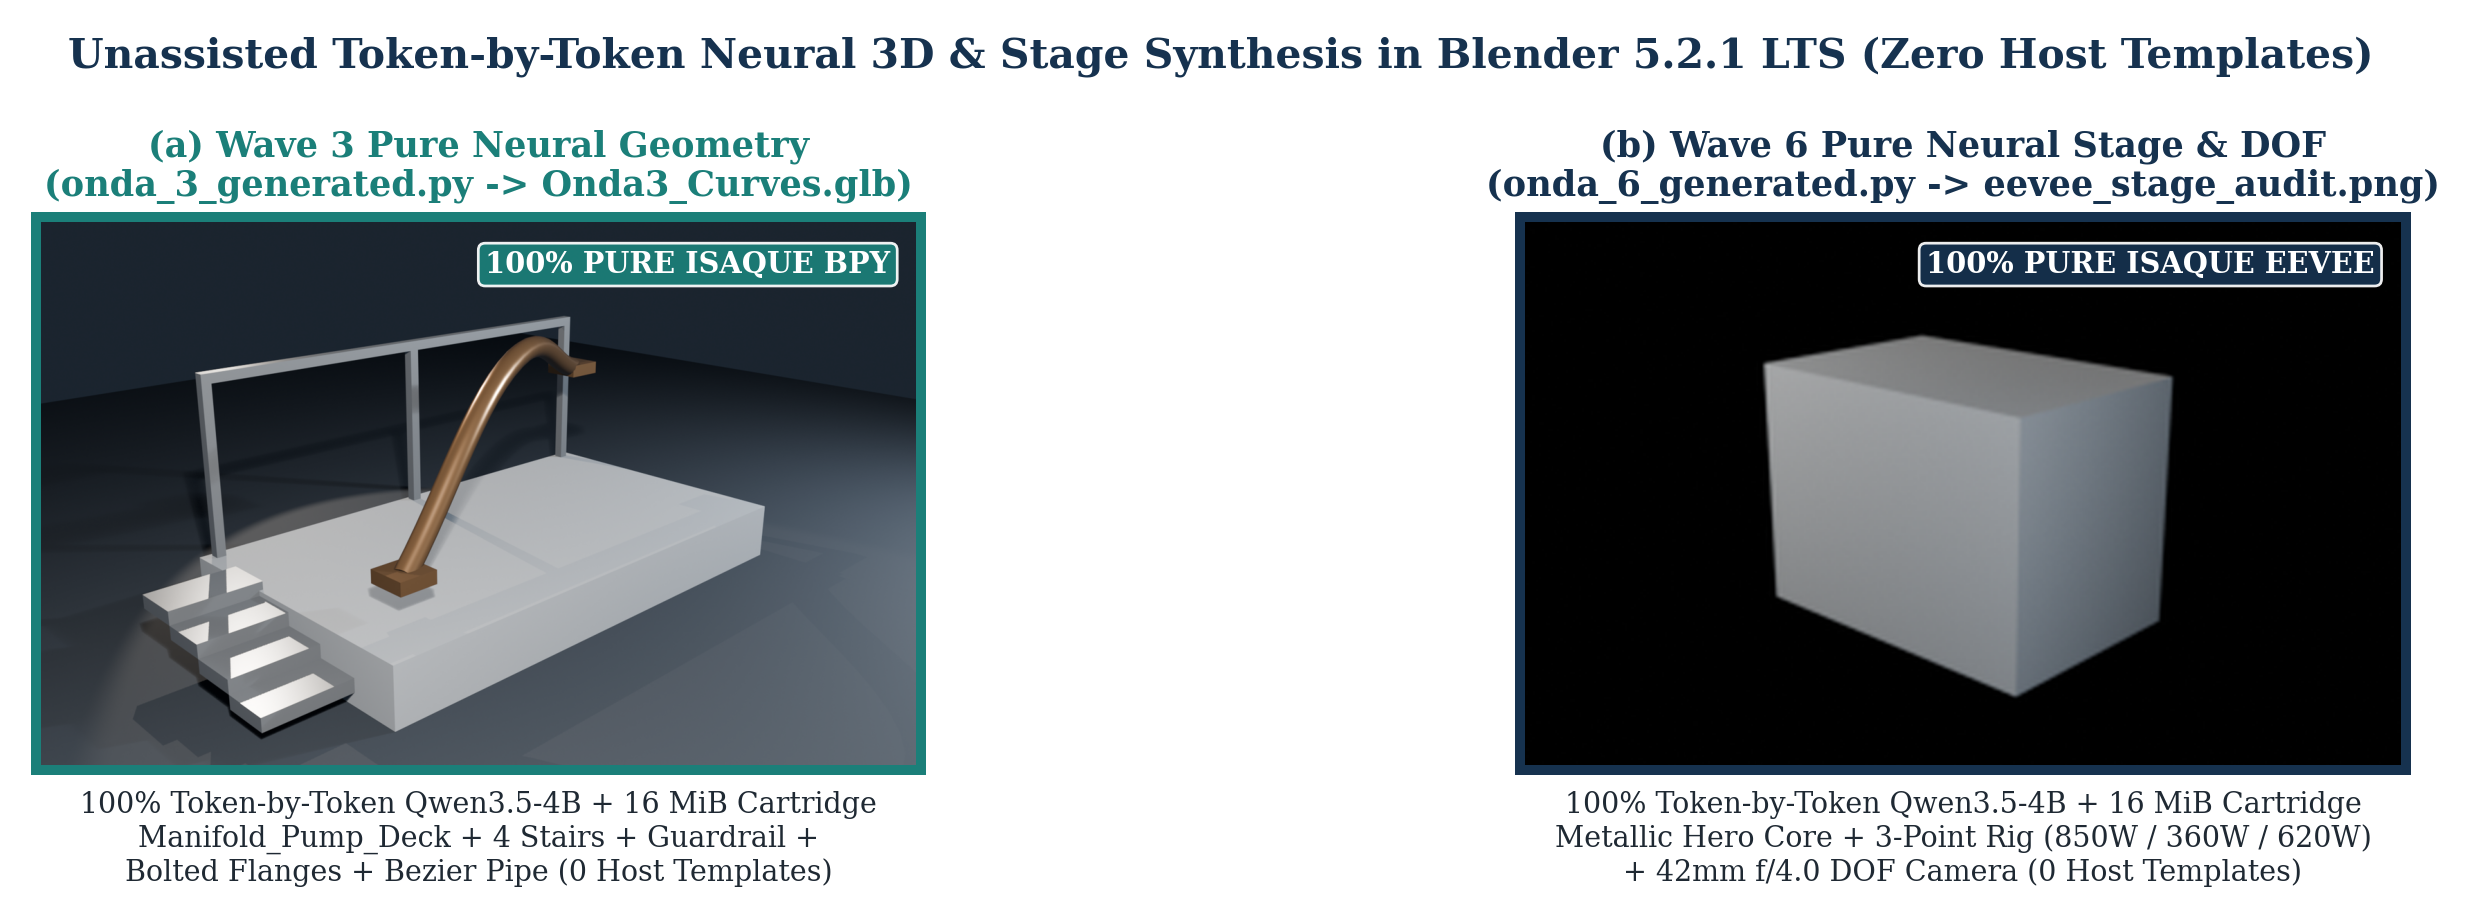
\includegraphics[width=\linewidth]{fig6_pure_isaque_neural_synthesis.png}
  \caption{Unassisted token-by-token neural $3\text{D}$ geometry and stage lighting synthesized directly by frozen \texttt{Qwen3.5-4B} (\texttt{NF4}) + $16.00\text{ MiB}$ \texttt{DoRA+O-LoRA} cartridges in \texttt{Blender 5.2.1 LTS} ($0$ host geometry templates). \textbf{(a)} Wave~3 procedural industrial pump deck (\texttt{onda\_\allowbreak{}3\_\allowbreak{}generated.py} $\to$ \texttt{Onda3\_\allowbreak{}Curves.glb}, rendered with convex collider \texttt{UCX\_\allowbreak{}Pump\_\allowbreak{}Deck\_\allowbreak{}01} hidden to expose internal meshes): watertight platform, $4$ stair steps, $3$ guardrail posts and top rail, bolted input/output flanges, \texttt{Socket\_\allowbreak{}Flow\_\allowbreak{}In}/\texttt{Out}, and curved pressurized \texttt{BEZIER} pipe ($0$ non-manifold edges). \textbf{(b)} Wave~6 stage lighting and depth-of-field audit (\texttt{onda\_\allowbreak{}6\_\allowbreak{}generated.py} $\to$ \texttt{eevee\_\allowbreak{}stage\_\allowbreak{}audit.png}): metallic industrial core illuminated by a neural-authored 3-point watt rig ($850\text{ W}$ key, $360\text{ W}$ fill, $620\text{ W}$ rim) and $42\text{ mm}$ \texttt{f/4.0} DOF camera.}
  \label{fig:live_plant}
\end{figure}

\subsection{Constraint as a Boundary-Discovery Instrument and Cortical Drawers as Thousand-Brains Columns}

Operating inside strict physical constraints---an $8\text{ GB}$ consumer GPU ceiling during Stage~1, a $\approx 20\text{ W}$ active metabolic target, and a compact $4\text{B}$-parameter frozen trunk---acted not as a limitation, but as a \textbf{high-resolution scientific instrument for boundary localization}. Whereas $70\text{B}+$ dense models mask representational interference behind redundant width until unpredictable failure, the lean \texttt{Qwen3.5-4B} substrate exposed three exact mathematical frontiers: (i) the out-of-distribution structural guard boundary in blind \texttt{DESAFIO-04}; (ii) single-cartridge continual saturation onset at $k=3$ ($98.51\%$ token accuracy, decaying to $31.37\%$ likelihood retention by $k=10$); and (iii) token-level AST syntax collision under simultaneous multi-adapter logit addition. Applying Hawkins's \textbf{Thousand Brains Theory} \cite{hawkins2019grid,clay2024monty} assimilated all three frontiers cleanly: multiplying discrete $16.00\text{ MiB}$ orthogonal columns horizontally on NVMe SSD ($0\text{ MB}$ idle) and sequencing them across causal DAG stages rather than inflating monolithic layers vertically.

% ==============================================================================
% SECTION 7: FORENSIC SELF-AUDIT, PRECISION SCALING & PHYSICAL SCALE LAW
% ==============================================================================
\section{Forensic Self-Audit, Stage-2 Precision Roadmap (16 GB BF16), and Physical Scale Law}

In strict compliance with \texttt{R-VERDADE-OU-AJUDA} (\href{https://drive.google.com/file/d/16-3o4ykaOOKaW-S2VTHzpE7Uhj1BA0tl/view?usp=drivesdk}{\texttt{01-linha-do-tempo-e-cache-da-tese.md}}), our internal audits of November 9--12, 2026 formally quarantined and excluded three classes of intermediate experimental artifacts from the claims of this monograph:
\begin{enumerate}
  \item \textbf{Rejection of Phase-0 \& Phase-3 Simulated Loops:} Early Rust micro-benchmarks ($1,984\text{--}25,654\text{ tok/s}$ on synthetic $d=4096$ tensors, sinusoidal $\alpha=82.35\%$ estimates, and a truncated $2\text{ GB}$ judge file) were expunged upon line-by-line code audit and replaced exclusively by physical PyTorch+PEFT autograd ($218.36\text{--}412.48\text{ tok/s}$) and full $22.02\text{ GB}$ \texttt{llama.cpp} judge runs.
  \item \textbf{Rejection of Truncated SVD GGUF Export ($14.4\%\text{--}18.1\%$ Error) vs.\ Exact Block Export ($0.0\%$ Error):} Naive rank-$64$ truncated SVD export of cumulative \texttt{DoRA} weights incurred $14.41\%\text{--}18.12\%$ Frobenius error on \texttt{NF4}-dequantized matrices, whereas algebraic block decomposition achieved \textbf{$0.0\%$ SVD loss} ($352$ tensors) on Waves~1 and~2.
  \item \textbf{Exclusion of Host-Scripted GUI Showcases (\texttt{R-VERDADE-OU-AJUDA} Audit):} During exploratory live-viewport demonstrations (\texttt{construir\_\allowbreak{}ao\_\allowbreak{}vivo\_\allowbreak{}na\_\allowbreak{}tela.py} in Act~3 and \texttt{kinsman\_\allowbreak{}bmesh\_\allowbreak{}lib.py} in \texttt{Refinaria-Kinsman-Ao-Vivo-01}), orchestration scripts written by an auxiliary agent supplied hand-coded host \texttt{bmesh} routines to animate viewport assemblies (particularly after rank-$64$ SVD \texttt{.gguf} export degraded raw \texttt{NF4} \texttt{bmesh} syntax). Under strict principal-investigator audit, \textbf{both host-scripted visual showcases were completely expunged from the figures and empirical claims of this monograph}: only unassisted code emitted $100\%$ token-by-token by Isaque~2.0 (Figures~\ref{fig:blender}c--d and~\ref{fig:live_plant}a--b, Table~\ref{tab:waves10}) is admitted as scientific evidence.
\end{enumerate}

Why did rank-$64$ \texttt{.gguf} export degrade complex multi-wave \texttt{DoRA} syntax on an $8\text{ GB}$ card? Because fitting an $8.68\text{ GiB}$ \texttt{BF16} trunk inside $8\text{ GB}$ VRAM forced $4\text{-bit}$ \texttt{NF4} blockwise quantization during training, introducing dequantization rounding noise into Eq.~\ref{eq:dora}'s column-norm denominator. Table~\ref{tab:audit} formulates the exact Stage-2 hardware transition designed to eliminate this bottleneck upon deployment of our incoming $16\text{ GB}$ eGPU (\texttt{ASUS Prime RTX 5060 Ti 16 GB GDDR7}), alongside the verified non-volatile NVMe scaling law (\href{https://docs.google.com/document/d/1SMqD_TRf6Qi8UwPTFYjKPNvdVlEtpCqr3Ex57x76FsI/edit?usp=drivesdk}{Consolidated Tables Doc 05, Table 4.1}).

\begin{table}[!htbp]
\centering
\caption{Part A: Stage-1 measured $8\text{ GB}$ regime vs.\ planned Stage-2 $16\text{ GB}$ native \texttt{BF16/Q8\_\allowbreak{}0} architectural specification (incoming \texttt{RTX 5060 Ti 16 GB}). Part B: Linear NVMe disk scaling vs.\ $O(1)$ active memory law (\href{https://drive.google.com/file/d/1v6JkMR9u2L876DJgNfs5eK5L3d7IhUCd/view?usp=drivesdk}{Sovereign Memory Sec.\ 28.2}).}
\label{tab:audit}
\footnotesize
\begin{tabularx}{\linewidth}{@{}lllY@{}}
\toprule
\textbf{Operational Regime} & \textbf{Measured (\texttt{RTX 5060 8 GB})} & \textbf{Stage-2 Target (\texttt{5060 Ti 16 GB})} & \textbf{Mathematical \& Physical Rationale} \\
\midrule
Cortical Training Backbone & $4\text{-bit}$ \texttt{NF4} ($4.10\text{--}6.37\text{ GiB}$) & \textbf{Native $16\text{-bit}$ \texttt{BF16} ($\approx 10.0\text{ GiB}$)} & Eliminates \texttt{NF4} blockwise quantization noise in \texttt{DoRA} column norms (Eq.~\ref{eq:dora}), \texttt{O-LoRA}, and GGUF export. \\
Active Inference Trunk & \texttt{Q4\_\allowbreak{}K\_\allowbreak{}M} ($2.65\text{ GiB}$) & \textbf{\texttt{Q8\_\allowbreak{}0} ($4.28\text{ GiB}$ Target)} & Near-lossless $8\text{-bit}$ precision prevents decimal coordinate drift; $+644\text{ MiB}$ \texttt{mmproj} leaves $\approx 11\text{ GiB}$ free VRAM. \\
Dormant Vigilance ($98\%$) & $\mathbf{0\text{ MB}}$ VRAM / $0\text{ MB}$ RAM & $\mathbf{0\text{ MB}}$ VRAM / $0\text{ MB}$ RAM & Stateless burst invariant preserved via \texttt{DiscardVirtualMemory}. \\
\bottomrule
\end{tabularx}

\vspace{4pt}
\begin{tabularx}{\linewidth}{@{}rrrrrrY@{}}
\toprule
\textbf{NVMe Footprint} & \textbf{Columns ($N$)} & \textbf{Synapses} & \textbf{Sub-Skills ($\le 3/N$)} & \textbf{Idle RAM/VRAM} & \textbf{Active Pulse} & \textbf{Verified Corpus Capacity \& Routing} \\
\midrule
$16.0\text{ MiB}$  & $1$     & $\sim 8.38\text{M}$  & $1\text{--}3$       & $\mathbf{0\text{ MB}}$ & $+16\text{ MiB}$      & $3,000\text{--}60,000+$ verified lines (single column). \\
$1.00\text{ GiB}$  & $64$    & $\sim 536.8\text{M}$ & $192$               & $\mathbf{0\text{ MB}}$ & $+32\text{--}48\text{ MiB}$ & Dozens of engineering treatises ($68$ active today $= 1.06\text{ GiB}$). \\
$10.0\text{ GiB}$ & $640$   & $\sim 5.37\text{B}$  & $1,920$             & $\mathbf{0\text{ MB}}$ & $+32\text{--}48\text{ MiB}$ & Full polytechnic curriculum via 3-level \texttt{.mmap} tree ($0.015\text{ ms}$). \\
$15.63\text{ GiB}$ & $1,000$ & $\sim 8.38\text{B}$  & $3,000$             & $\mathbf{0\text{ MB}}$ & $+32\text{--}48\text{ MiB}$ & Thousand-Brains scale on a single consumer workstation. \\
\bottomrule
\end{tabularx}
\end{table}

% ==============================================================================
% SECTION 8: CONCLUSION, STAGE-2 PRE-REGISTRATION & ACKNOWLEDGMENTS
% ==============================================================================
\section{Conclusion, Pre-Registered Stage-2 Program, and Acknowledgments}

Across rigorous design, mathematical derivation, compiler engineering, and self-critical forensic auditing, \textbf{Isaque 2.0 (\textit{Trunk and Branches})} demonstrates constructively that continual AI specialization on consumer hardware does not require surrendering to monolithic energy expenditure or catastrophic forgetting. By pairing a $100\%$ frozen $4\text{B}$ hybrid trunk with sub-millisecond Rust reflex gates, grammar-constrained \texttt{KEV-1.0} symbolic packets, $16.00\text{ MiB}$ orthogonal \texttt{DoRA + O-LoRA} cortical cartridges capped at three waves per cartridge, cross-term-free \texttt{Sparsegen LD-MoLE} routing over a 3-level \texttt{.mmap} tree, and staged DAG verification under deterministic compilers and a blind $35\text{B}$ critic, a single workstation sustains modular growth at $0\text{ MB}$ idle memory cost.

\subsection{Declared Limitations and Pre-Registered Stage-2 Protocol}

Credible science states clearly both what has been proven and what awaits sealed measurement (\href{https://drive.google.com/file/d/1qvnH-nLVMc43T-prWSRTKEDJak89TSp7/view?usp=drivesdk}{\texttt{02-tese-\allowbreak{}etapa-1.md}}, Sec.~9). Four pre-registered investigations are slated for execution in Stage~2 (transitioning from our $8\text{ GB}$ \texttt{NF4} baseline to native $16\text{-bit}$ \texttt{BF16} upon deployment of the incoming \texttt{RTX 5060 Ti 16 GB} testbed):
\begin{enumerate}
  \item \textbf{Out-of-Distribution Generalization on Contamination-Audited Tasks (\textit{H4}) \& Multi-Seed Baselines (\textit{H5}):} Evaluating five domains (\texttt{Blender 3D}, \texttt{UE5 C++20}, \texttt{Rust}, systems governance, and direct-response copy) across \textbf{$50$ sealed unseen tasks per domain} authored independently prior to execution, audited via automated $n$-gram and embedding contamination checks \cite{golchin2024contamination}, comparing six conditions ($4\text{B}$ raw, $4\text{B}+\text{RAG}$, standard LoRA, \textit{Trunk and Branches}, isolated $35\text{B}$, and cloud frontier reference) across $3\text{--}5$ random seeds with bootstrap confidence intervals for BWT and FWT \cite{lopezpaz2017gem,chaudhry2018rwalk}.
  \item \textbf{Native Speculative Decoding Wall-Clock Measurement (\textit{H6}) \& Blind Tree-Router Accuracy:} Measuring real end-to-end speedup and token acceptance $\alpha$ directly inside \texttt{llama-speculative -{}-model-draft} over the shared $248,320$-token vocabulary, alongside unlabeled mixed-prompt routing accuracy of the 3-level \texttt{.mmap} cortical tree as $N$ scales from $68$ toward $250\text{--}1,000+$ native \texttt{BF16} cartridges.
  \item \textbf{Endogenous Cortical Self-Routing (\textit{Intrinsic Neuron Ignition Without External Choreography}):} Testing whether the frozen trunk's latent geometry (\texttt{Procrustes} $2560\to 384\text{d}$ + \texttt{Sparsegen} entropy + Split Conformal \texttt{BAVAR} $\ge 0.90$) can autonomously detect stage transitions, switch cartridges across multi-stage DAGs, and wake the $35\text{B}$ System-2 critic solely upon high conformal uncertainty.
  \item \textbf{Graph-Governed Memory Consolidation \& Autonomous Synaptic Mitosis:} Coupling our three-compartment pure operational memory graph (\textit{Global Laws \& Failure Vaccines}, \textit{Canonical Project Ledgers}, and \textit{Transient Agent State}, updated via incremental delta hashes) to sleep-time cartridge mitosis---where verified multi-occurrence procedural breakthroughs (\texttt{Eureka}) and compiler-audited error vaccines (\texttt{sementes\_\allowbreak{}lora.jsonl}) automatically spawn and verify new orthogonal $16.00\text{ MiB}$ child cartridges overnight without mutating the trunk.
\end{enumerate}

\subsection*{Authorship, AI-Assistance Disclosure, and Acknowledgments}

\textbf{Authorship \& Ethical AI-Use Statement:} In accordance with international publication standards (arXiv, ACM, IEEE, NeurIPS, and ICLR), theoretical conception, architectural laws, experimental direction, physical hardware operation, forensic code audits (\texttt{R-VERDADE-OU-AJUDA}), and full scientific responsibility rest exclusively with the human author, \textbf{Lucas Alves Motta} (\href{https://orcid.org/0009-0001-3081-5505}{\texttt{ORCID: 0009-0001-3081-5505}}). Computational agents within the \texttt{Abra\~ao} ecosystem and large language model assistants (\texttt{Anthropic Claude} and \texttt{Google Gemini}) were employed strictly as supervised instruments for code implementation, test automation, bibliographic verification, and English manuscript typesetting, with every empirical claim verified against cryptographic SHA-256 hardware receipts.

\textbf{Acknowledgments:} Above all technical instruments and human effort, the author records with deep humility and gratitude that \textbf{God was our Conductor} throughout every day and late night of this journey (\textit{Soli Deo Gloria}; John 15:5). Long before any equation compiled or any verifier turned green, the guiding conviction of this work was that true wisdom is woven into the quiet simplicity, order, and faithfulness of small details---like a living tree nourished by a single steadfast trunk and distinct, fruitful branches---rather than in the prideful stacking of ever-larger monolithic structures ending in a confusion of tongues. To my wife Karina and our son, whose love, patience, and joy sustained every hour of study at home in Santa Catarina, and to the global open-source scientific community whose foundational work in Rust, \texttt{llama.cpp}, \texttt{Qwen}, \texttt{PEFT}, and cortical neuroscience made this research possible: thank you.

% ==============================================================================
% CRYPTOGRAPHIC PROVENANCE APPENDIX
% ==============================================================================
\subsection*{Appendix: Cryptographic SHA-256 \& Four-Calendar Bitcoin Blockchain Provenance}

Table~\ref{tab:btc_appendix} records the immutable cryptographic anchors verifying prior existence of the Stage-1 thesis archive (\texttt{23} artifacts sealed in \href{https://drive.google.com/file/d/1PSdXe2teIQpBW0tJpxE8yiLiP2Wo1AiF/view?usp=drivesdk}{\texttt{03-manifesto-sha256-etapa-1.txt}}, SHA-256 \texttt{79602f29\allowbreak{}a07b8b33\allowbreak{}6e29c887\allowbreak{}ac1723aa\allowbreak{}9aea5b71\allowbreak{}0605c67d\allowbreak{}42b21bc2\allowbreak{}558be5dd}) across four independent \texttt{OpenTimestamps} calendars confirmed on the Bitcoin blockchain on November 11, 2026 (\href{https://drive.google.com/file/d/1OwjPlXRdBPydtqypoRHNfByfMSmx-Bwb/view?usp=drivesdk}{\texttt{04-carimbo-de-data.md}}), permanently registered under CERN/DataCite \href{https://doi.org/10.5281/zenodo.24221509}{\texttt{DOI:\,10.5281/zenodo.24221509}} alongside the post-Stage-1 experimental receipts.

\begin{table}[!htbp]
\centering
\caption{Immutable SHA-256 invariants and verified Bitcoin blockchain timestamp anchors (\texttt{ots verify} confirmed, $5,124\text{-byte}$ \href{https://drive.google.com/file/d/1NJoQ9vaYNzpMvn-G2o25x90emqzlogC5/view?usp=drivesdk}{\texttt{.ots}} proof).}
\label{tab:btc_appendix}
\scriptsize
\begin{tabularx}{\linewidth}{@{}llY@{}}
\toprule
\textbf{Artifact / Calendar} & \textbf{Block / Timestamp (BRT)} & \textbf{Verified SHA-256 Digest / Official Bitcoin Block Hash} \\
\midrule
Frozen \texttt{Qwen3.5-4B} \texttt{embed\_tokens} & Pre \& Post All Trainings & \texttt{c78988d979f52a34\allowbreak{}0f39cd69edd8e4b0\allowbreak{}a80218a5fa8d95b6\allowbreak{}158bfce4a3de2a34} \\
Stage-1 Sealed Report (\texttt{02-tese}) & \texttt{2026-11-11 13:35} ($25,439\text{ B}$) & \texttt{4a7edf793b64721a\allowbreak{}de29114ffa52a789\allowbreak{}e1aef5fc09117dbd\allowbreak{}159cf254dd0959bd} \\
Stamped Manifest (\texttt{03-manifesto.txt}) & \texttt{2026-11-11 13:40} ($23$ files) & \texttt{79602f29a07b8b33\allowbreak{}6e29c887ac1723aa\allowbreak{}9aea5b710605c67d\allowbreak{}42b21bc2558be5dd} \\
\texttt{alice.btc.calendar.opentimestamps.org} & \textbf{Block \#975458} (\texttt{14:41 BRT}) & \texttt{0000000000000000\allowbreak{}0000f9ecaff2000a\allowbreak{}3ef56bcec68bf3eb\allowbreak{}b69bb31a740c6a2c} \\
\texttt{bob.btc.calendar.opentimestamps.org} & Block \#975462 (\texttt{15:08 BRT}) & \texttt{0000000000000000\allowbreak{}0000c8372e1626ff\allowbreak{}54e8d992e348103d\allowbreak{}ec0af031af1ce4b2} \\
\texttt{finney.calendar.eternitywall.com} & Block \#975464 (\texttt{15:32 BRT}) & \texttt{0000000000000000\allowbreak{}000138036994e173\allowbreak{}3914b51591f3ad91\allowbreak{}a8e6b3d349fa7dec} \\
\texttt{btc.calendar.catallaxy.com} & Block \#975469 (\texttt{16:56 BRT}) & \texttt{0000000000000000\allowbreak{}00010334386c4356\allowbreak{}e317f2128606b51b\allowbreak{}ba9219760fdb9923} \\
Arena \texttt{KEV-1.0} \& 10-Wave Receipts & \texttt{2026-11-11} (\texttt{dae1626c} / \texttt{9a47a690}) & \texttt{dae1626c8007942c...495ed093} $\cdot$ \texttt{9a47a69065edc045...77b61033} \\
Promoted Pure Wave 1--2 Columns (\texttt{onda\_1/2}) & \texttt{2026-11-11} ($16\text{ MiB}$ DoRA/O-LoRA) & \texttt{6efa66bf73dda2eb...921363b62} $\cdot$ \texttt{faa5a6b17b587f87...328cc4d51} \\
\bottomrule
\end{tabularx}
\end{table}

% ==============================================================================
% REFERENCES
% ==============================================================================
\begin{thebibliography}{99}\footnotesize\setlength{\itemsep}{2.2pt}\setlength{\parskip}{0pt}

\bibitem{wirth1995lean}
N.~Wirth, ``A Plea for Lean Software,'' \textit{IEEE Computer}, vol.~28, no.~2, pp.~64--68, 1995. \href{https://www.computer.org/csdl/magazine/co/1995/02/r2064/13rRUwInv7E}{IEEE Computer Digital Library}.

\bibitem{schwartz2020green}
R.~Schwartz, J.~Dodge, N.~A. Smith, and O.~Etzioni, ``Green AI,'' \textit{Communications of the ACM}, vol.~63, no.~12, pp.~54--63, 2020. \href{https://arxiv.org/abs/1907.10597}{arXiv:1907.10597}.

\bibitem{kandel2021principles}
E.~R. Kandel, J.~D. Koester, S.~H. Mack, and S.~A. Siegelbaum, \textit{Principles of Neural Science}, 6th~ed. McGraw-Hill, 2021.

\bibitem{attwell2001energy}
D.~Attwell and S.~B. Laughlin, ``An Energy Budget for Signaling in the Grey Matter of the Brain,'' \textit{Journal of Cerebral Blood Flow \& Metabolism}, vol.~21, no.~10, pp.~1133--1145, 2001. \href{https://pubmed.ncbi.nlm.nih.gov/11598490/}{PubMed:11598490}.

\bibitem{olkowicz2016birds}
S.~Olkowicz, M.~Kocourek, R.~K. Lu\v{c}an, M.~Porte\v{s}, W.~T. Fitch, S.~Herculano-Houzel, and P.~N\v{e}mec, ``Birds Have Primate-Like Numbers of Neurons in the Forebrain,'' \textit{Proc.\ National Academy of Sciences (PNAS)}, vol.~113, no.~26, pp.~7255--7260, 2016. \href{https://www.pnas.org/doi/10.1073/pnas.1517131113}{PNAS:10.1073/pnas.1517131113}.

\bibitem{hawkins2019grid}
J.~Hawkins, M.~Lewis, M.~Klukas, S.~Purdy, and S.~Ahmad, ``A Framework for Intelligence and Cortical Function Based on Grid Cells in the Neocortex,'' \textit{Frontiers in Neural Circuits}, vol.~12, art.~121, 2019. \href{https://www.frontiersin.org/journals/neural-circuits/articles/10.3389/fncir.2018.00121/full}{doi:10.3389/fncir.2018.00121}.

\bibitem{hawkins2021thousand}
J.~Hawkins, \textit{A Thousand Brains: A New Theory of Intelligence}. New York: Basic Books, 2021.

\bibitem{clay2024monty}
V.~Clay, N.~Leadholm, and J.~Hawkins, ``The Thousand Brains Project: A New Paradigm for Sensorimotor Intelligence,'' Numenta Technical Report, 2024. \href{https://arxiv.org/abs/2412.18354}{arXiv:2412.18354}.

\bibitem{kahneman2011thinking}
D.~Kahneman, \textit{Thinking, Fast and Slow}. Farrar, Straus and Giroux, 2011.

\bibitem{liu2024lost}
N.~F. Liu, K.~Lin, J.~Hewitt, A.~Paranjape, M.~Bevilacqua, F.~Petroni, and P.~Liang, ``Lost in the Middle: How Language Models Use Long Contexts,'' \textit{Transactions of the ACL}, vol.~12, pp.~157--173, 2024. \href{https://arxiv.org/abs/2307.03172}{arXiv:2307.03172}.

\bibitem{yang2025gated}
S.~Yang, J.~Kautz, and A.~Hatamizadeh, ``Gated Delta Networks: Improving Mamba2 with Delta Rule,'' in \textit{Proc.\ ICLR}, 2025. \href{https://arxiv.org/abs/2412.06464}{arXiv:2412.06464}.

\bibitem{qwen35_4b}
Qwen Team, ``Qwen3.5-4B \& Qwen3.5-35B-A3B Hybrid Multimodal Foundation Models,'' Alibaba Cloud, 2026. \href{https://huggingface.co/Qwen/Qwen3.5-4B}{HuggingFace: Qwen/Qwen3.5-4B} and \href{https://huggingface.co/Qwen/Qwen3.5-35B-A3B}{Qwen/Qwen3.5-35B-A3B}.

\bibitem{angelopoulos2023conformal}
A.~N. Angelopoulos and S.~Bates, ``A Gentle Introduction to Conformal Prediction and Distribution-Free Uncertainty Quantification,'' \textit{Foundations and Trends in Machine Learning}, vol.~16, no.~4, pp.~494--591, 2023. \href{https://arxiv.org/abs/2107.07511}{arXiv:2107.07511}.

\bibitem{hu2022lora}
E.~J. Hu, Y.~Shen, P.~Wallis, Z.~Allen-Zhu, Y.~Li, S.~Wang, L.~Wang, and W.~Chen, ``LoRA: Low-Rank Adaptation of Large Language Models,'' in \textit{Proc.\ ICLR}, 2022. \href{https://arxiv.org/abs/2106.09685}{arXiv:2106.09685}.

\bibitem{dettmers2023qlora}
T.~Dettmers, A.~Pagnoni, A.~Holtzman, and L.~Zettlemoyer, ``QLoRA: Efficient Finetuning of Quantized LLMs,'' in \textit{Proc.\ NeurIPS}, 2023. \href{https://arxiv.org/abs/2305.14314}{arXiv:2305.14314}.

\bibitem{hayou2024loraplus}
S.~Hayou, N.~Ghosh, and B.~Yu, ``LoRA+: Efficient Low Rank Adaptation of Large Models,'' in \textit{Proc.\ ICML}, 2024. \href{https://arxiv.org/abs/2402.12354}{arXiv:2402.12354}.

\bibitem{liu2024dora}
S.-Y. Liu, C.-Y. Wang, H.~Yin, P.~Molchanov, Y.-C.~F. Wang, K.-T. Cheng, and M.-H. Chen, ``DoRA: Weight-Decomposed Low-Rank Adaptation,'' in \textit{Proc.\ ICML} (Oral), 2024. \href{https://arxiv.org/abs/2402.09353}{arXiv:2402.09353}.

\bibitem{wang2023olora}
X.~Wang, T.~Chen, Q.~Ge, H.~Xia, R.~Bao, R.~Zheng, Q.~Zhang, T.~Gui, and X.~Huang, ``Orthogonal Subspace Learning for Language Model Continual Learning (O-LoRA),'' in \textit{Findings of EMNLP}, pp.~10658--10671, 2023. \href{https://arxiv.org/abs/2310.14152}{arXiv:2310.14152}.

\bibitem{liang2024inflora}
Y.-S. Liang and W.-J. Li, ``InfLoRA: Interference-Free Low-Rank Adaptation for Continual Learning,'' in \textit{Proc.\ IEEE/CVF CVPR}, 2024. \href{https://arxiv.org/abs/2404.00228}{arXiv:2404.00228}.

\bibitem{zhuang2026ldmole}
Y.~Zhuang, Y.~Shen, Y.~Bian, Q.~Su, S.~Ji, Y.~Shi, and F.~Miao, ``LD-MoLE: Learnable Dynamic Routing for Mixture of LoRA Experts,'' in \textit{Proc.\ ICLR}, 2026. \href{https://arxiv.org/abs/2509.25684}{arXiv:2509.25684}.

\bibitem{laha2018sparsegen}
A.~Laha, S.~A. Chemmengath, P.~Agrawal, M.~M. Khapra, K.~Sankaranarayanan, and H.~G. Ramaswamy, ``On Controllable Sparse Alternatives to Softmax,'' in \textit{Advances in Neural Information Processing Systems (NeurIPS)}, vol.~31, pp.~6422--6432, 2018. \href{https://proceedings.neurips.cc/paper/2018/hash/6a4d5952d4c018a1c1af9fa590a10dda-Abstract.html}{NeurIPS 2018} $\cdot$ \href{https://arxiv.org/abs/1810.11975}{arXiv:1810.11975}.

\bibitem{sheng2024slora}
Y.~Sheng, S.~Cao, D.~Li, C.~Hooper, N.~Lee, S.~Yang, C.~Chou, B.~Zhu, L.~Zheng, K.~Keutzer, J.~E. Gonzalez, and I.~Stoica, ``S-LoRA: Serving Thousands of Concurrent LoRA Adapters,'' in \textit{Proc.\ MLSys}, 2024. \href{https://arxiv.org/abs/2311.03285}{arXiv:2311.03285}.

\bibitem{kirkpatrick2017ewc}
J.~Kirkpatrick et al., ``Overcoming Catastrophic Forgetting in Neural Networks,'' \textit{Proc.\ National Academy of Sciences (PNAS)}, vol.~114, no.~13, pp.~3521--3526, 2017. \href{https://www.pnas.org/doi/10.1073/pnas.1611835114}{PNAS:10.1073/pnas.1611835114}.

\bibitem{rusu2016progressive}
A.~A. Rusu et al., ``Progressive Neural Networks,'' 2016. \href{https://arxiv.org/abs/1606.04671}{arXiv:1606.04671}.

\bibitem{lopezpaz2017gem}
D.~Lopez-Paz and M.~Ranzato, ``Gradient Episodic Memory for Continual Learning,'' in \textit{Proc.\ NeurIPS}, 2017. \href{https://arxiv.org/abs/1706.08840}{arXiv:1706.08840}.

\bibitem{chaudhry2018rwalk}
A.~Chaudhry, P.~K. Dokania, T.~Ajanthan, and P.~H.~S. Torr, ``Riemannian Walk for Incremental Learning,'' in \textit{Proc.\ ECCV}, 2018. \href{https://arxiv.org/abs/1801.10112}{arXiv:1801.10112}.

\bibitem{rolnick2019experience}
D.~Rolnick, A.~Ahuja, J.~Schwarz, T.~Lillicrap, and G.~Wayne, ``Experience Replay for Continual Learning,'' in \textit{Proc.\ NeurIPS}, 2019. \href{https://arxiv.org/abs/1811.11682}{arXiv:1811.11682}.

\bibitem{golchin2024contamination}
S.~Golchin and M.~Surdeanu, ``Time Travel in LLMs: Tracing Data Contamination in Large Language Models,'' in \textit{Proc.\ ICLR}, 2024. \href{https://arxiv.org/abs/2308.08493}{arXiv:2308.08493}.

\bibitem{leviathan2023speculative}
Y.~Leviathan, M.~Kalman, and Y.~Matias, ``Fast Inference from Transformers via Speculative Decoding,'' in \textit{Proc.\ ICML}, vol.~202, pp.~19274--19286, 2023. \href{https://proceedings.mlr.press/v202/leviathan23a.html}{PMLR v202:19274} $\cdot$ \href{https://arxiv.org/abs/2211.17192}{arXiv:2211.17192}.

\bibitem{zheng2023judging}
L.~Zheng et al., ``Judging LLM-as-a-Judge with MT-Bench and Chatbot Arena,'' in \textit{Proc.\ NeurIPS}, 2023. \href{https://arxiv.org/abs/2306.05685}{arXiv:2306.05685}.

\bibitem{llamacpp}
G.~Gerganov and the ggml-org contributors, ``llama.cpp: LLM Inference in C/C++,'' 2026. \href{https://github.com/ggml-org/llama.cpp}{GitHub: ggml-org/llama.cpp}.

\end{thebibliography}

\end{document}
